%\documentclass[preprint]{aastex}  % USE THIS TO MAKE BIB, THEN FORMAT USING EMULATEAPJ
\documentclass[twocolumn,apj,numberedappendix]{emulateapj}
\shorttitle{Fringe-Rate Filtering}
\shortauthors{Parsons, et al.}

\usepackage{amsmath}
\usepackage{graphicx}
\usepackage[figuresright]{rotating}
%\usepackage{rotating}
\usepackage{natbib}
%\usepackage{pdflscape}
%\usepackage{lscape}
\citestyle{aa}

\def\b{\mathbf{b}}
\def\k{\mathbf{k}}
\def\r{\mathbf{r}}
\def\q{\mathbf{q}}
\def\b{\mathbf{b}}
\def\kp{\mathbf{k}^\prime}
\def\kpp{\mathbf{k}^{\prime\prime}}
\def\V{\mathbb{V}}
\def\At{\tilde{A}}
\def\Vt{\tilde{V}}
\def\Tt{\tilde{T}}
\def\tb{\langle T_b\rangle}
\newcommand{\vis}{\mathbf{v}}
\newcommand{\x}{\mathbf{x}}
\newcommand{\xhat}{\hat{\mathbf{x}}}
\newcommand{\A}{\mathbf{A}}
\newcommand{\N}{\mathbf{N}}
\newcommand{\rhat}{\hat{\mathbf{r}}}

\begin{document}
\title{Fringe-Rate Filtering}

\author{
Aaron R. Parsons\altaffilmark{1,2},
Adrian Liu\altaffilmark{1},
%James E. Aguirre\altaffilmark{3},
Zaki S. Ali\altaffilmark{1},
%David R. DeBoer\altaffilmark{2},
%Daniel C. Jacobs\altaffilmark{8},
%David F. Moore\altaffilmark{3},
%Jonathan C. Pober\altaffilmark{1},
% XXX if includes paper data, needs full author list
}

\altaffiltext{1}{Astronomy Dept., U. California, Berkeley, CA}
\altaffiltext{2}{Radio Astronomy Lab., U. California, Berkeley, CA}
%\altaffiltext{3}{Dept. of Physics and Astronomy, U. Pennsylvania, Philadelphia, PA}
%\altaffiltext{8}{School of Earth and Space Exploration, Arizona State U., Tempe, AZ}

\begin{abstract}
\end{abstract}

% XXX fringe weighting profile
% XXX delay spectrum not violated by freq-dependent fringe rate weights

% XXX Shorten introduction and move rest of material into a Background/FR filter basics section


\section{Introduction}

[XXX: Rework intro to make connection to 21cm more explicit.]

In any observation of the sky, integrating in time results in increased sensitivity.  Such increased sensitivity is particularly important in applications where instrumental noise levels are expected to be high compared to the faint signals that one seeks to measure.  As an example of this, in recent years multiple instruments have been built in an attempt to detect the redshifted $21\,\textrm{cm}$ line from the Epoch of Reionization\footnote{In this paper, we will frequently use $21\,\textrm{cm}$ interferometric arrays as example instruments with which to focus our discussion, and indeed, Sections XXX pertain only to such arrays.  However, we emphasize that the central idea of this paper---that fringe-rate filtering can be used to combine time-ordered data in a way that maximizes sensitivity---is one that should be widely applicable to any interferometer.}.  At the relevant redshifts ($z\sim 6$ to $20$), theoretical models suggest that this cosmological signal will be faint, on the order of $1\,\textrm{mK}$ in brightness temperature, while a typical instrument's system temperature is typically $\sim 100\,\textrm{K}$.  Long time-integrations are therefore crucial, and as a practical matter, this is often accomplished by accumulating time-samples, either in the image domain or in Fourier space.  In both cases, one is essentially making maps, which can be shown to be in principle a lossless method of data compression, and therefore an attractive method for realizing the increased sensitivity that time-integration provides.

The quest for increased sensitivity, however, has often led to instrumental designs that have made mapmaking algorithms rather unwieldy.  Consider first the possibility of accumulating time-samples in the image domain, again for the special case of a $21\,\textrm{cm}$ interferometer array.  To increase sensitivity, such arrays typically have wide fields-of-view and are configured to yield a large number of redundant baselines.  Over long time-integrations, imaging wide fields-of-view requires careful attention to curved-sky artifacts, which can become computationally expensive to control, particularly if the pixelization is taken to be extremely fine to avoid artifacts from gridding.  While a fine pixelization is necessary for mapmaking to be lossless (XXX: cite], this can become wasteful for interferometers with a large number of redundant baselines, in the sense that a large number of pixels are needed to store information about a small number of Fourier modes. [XXX: Make the connection in this last sentence a little clearer.]

Mapmaking in Fourier space (or more precisely, on the $uv$-plane) alleviates some of these problems.  Fourier space is a natural space for the accumulation of interferometric data, for there each baseline probes a relatively localized region.  It is therefore a particularly economical basis for accumulating interferometric data, especially if the final goal is to produce a spatial power spectrum, or other quantities that are ``native" to Fourier space.  However, gridding artifacts remain, and are even more troublesome when power spectrum estimation is considered in the context of rotation synthesis.  As the Earth rotates, baselines sample a series of points along tracks on the $uv$-plane.  Nearby points are almost perfectly correlated, and ought to be integrated coherently prior to the squaring step of any power spectrum measurement, while faraway points can only be combined statistically after squaring.  Unless one is willing to keep track of the level of correlation of every $uv$-point with every other $uv$-point, an arbitrary choice must be made as to how far away from each other two points can lie before they are considered incoherent.  Often, this choice is encapsulated by the $uv$-pixel size (particularly in calculations of power spectrum sensitivity XXX: cite), with samples falling in the same cells labeled as coherent, and those in different cells labeled as incoherent.  However, this can potentially lead to a loss of sensitivity in combining samples that straddle pixel boundaries.  While these obstacles can in principle be overcome, it is clear that extreme care must be taken in the mapmaking process to ensure that the full sensitivity of an interferometer array is realized.

% XXX "new method" was actually in Parsons Backer 2009.  
% XXX Might want to capture a more detailed working definition of fringe-rate filtering before starting to use the term
In this paper, we introduce a new method for combining time-ordered data---fringe-rate filtering---that avoids the aforementioned pitfalls while affording one the advantages traditionally reserved only when mapmaking.  The essential idea is that for an interferometer operating in a drift-scan observing mode, celestial sources of emission have predictable fringe-rates 

\begin{itemize}
\item For any instrument, important to integrate in time.  This is how you get sensitivity.
\item Historically (and what is conceptually the easiest) is to make a map and to bin there.
\item However, mapmaking is i) difficult, especially with the widefield instruments, ii) subject to artifacts and systematics such as gridding artifacts, iii) ``wasteful" for an interferometer array with high redundancy, since the image basis is not efficient if you're only measuring a small number of modes, iv) unnecessary if you're using an interferometer to measure a power spectrum.
\item For interferometers trying to measure a power spectrum, it'd be nice to be able to stay in the natural ``Fourier" space defined by an interferometer.
\item On the other hand, there are advantages to mapmaking that we want: i) coherent integrations in time, ii) the mitigation of systematics (such as polarization leakage), iii) the ability to down-weight data towards the edge of the primary beam (the instrument has already done that once, but an optimal inverse-variance weighted estimator needs to do it once again).  Not clear how to do that if one doesn't go to the image-domain.
\item In this paper, we introduce a method---fringe-rate filtering---that allows one to stay in visibility space but still get all the advantages of mapmaking.  The paper is geared towards drift-scan telescopes, although some of the lessons are also applicable to tracking telescopes.  The central idea is to Fourier-transform the time-series in order to sort the observations by fringe-rate, and then to enact a low-pass filter.  Since different parts of the sky have different interferometer fringe-rates, a careful tailoring of the filter can downweight different parts of the sky, allowing one to perform the downweightings towards the edge of the primary beam.
\item Fringe-rate space is particularly good for identifying high versus low signal-to-noise modes, because certain fringe-modes are physically impossible for true celestial emission (mention the super high azimuthal mode caveat here).  We can eliminate those modes.  This also makes it clear that time-averaging visibilities is not good.  Because it's a sinc in fringe-rate space, which has some high fringe-rate components.

\item Fringe-rate filters can be optimized to maximize sensitivity, assuming a noise power spectrum.  But they can also be used to help fight systematics.  As an example, 21cm arrays suffer from polarization leakage.  This can be particularly hard to fight because of the redundancy in the arrays.  Beam-sculpting, though, helps reduce this.  Specific to 21cm arrays, also show that we don't mess up delay-spectrum.
\item Other similar things in literature.  Richard's $m$-mode formalism made more explicit.  Optimal mapmaking.  Delay/DDR paper.  Also look at Andre's stuff.
\item Outline the paper.
\end{itemize}
Further details are supplied in Appendices A and B of \citet{parsons_et_al2013}.

%\begin{equation}
%\tilde{V}(\tau)=\int{W(\nu)\cdot S(\nu)\cdot V(\nu)e^{-2\pi i\nu\tau}~d\nu},
%\label{eq:dtransform}
%\end{equation}



\section{Overview of principle of fringe-rate filtering}
\label{sec:overview}
Generally, the interferometric response, $V$, for two antennas in a radio interferometer is described
by the measurement equation\footnote{In this section, we omit the instrumental noise contribution to the measured visibilities in order to avoid notational clutter.}
% XXX make this agree with Eq 2
\begin{equation}
V^b_\nu(t)=\int d\Omega \, {I_\nu(\rhat) A_\nu(\rhat,t) \exp \left[-i2\pi \frac{\nu}{c}  \mathbf{b}(t) \cdot \rhat\right]},
\end{equation}
where $I_\nu$ is the specific intensity of the sky in the direction $\rhat$,
$A_\nu$ is the geometric mean of the primary beam power patterns of the constituent antennas (henceforth known as ``the primary beam"), $\mathbf{ b}(t)$ is the baseline vector separating the two antennas in question (which is time-dependent since the baselines rotate with the Earth), and $\nu$ is the spectral
frequency.
%Interferometric responses (visibilities) for ground-based instruments are generally 
%a function of time, $t$, even for a static sky because the Earth's rotation makes the expression of $I$ 
%in topocentric coordinates a time-dependent quantity.
Here, we have adopted the convention that our coordinate system is fixed to the celestial sphere, because it will be convenient for our algebraic manipulations later. However, it is equally valid to understand the time-variation of the visibilities as arising from the movement of spatial structures through the primary beam and the fringes arising from a baseline that is fixed to a topocentric coordinate system. For drift-scan telescopes like PAPER, CHIME, or HERA, this view is particularly powerful because then the primary beam and the fringe pattern are locked to one another, and may together be considered an enveloped fringe pattern that gives rise
to time variation in $V_\nu(t)$ as the Earth rotates.

The rate at which angular structure on the sky moves relative to the fringe pattern---the \emph{fringe rate}---depends on the declination and hour angle. 
%
%Assuming that antenna positions are fixed to the Earth, the fringe pattern of an interferometer ---
%the variation in phase response across the sky --- is fixed in topocentric coordinates.  Hence, time
%variation in $V_\nu(t)$ can be regarded as resulting from the motion of spatial structures in $I$ through
%the fringe pattern and primary beam response pattern.  Moreover, for interferometers such as PAPER, CHIME, and HERA 
%% XXX others? cite here or before?
%that do not point, but instead drift-scan the sky as it rotates by, the primary beam response pattern and the
%phase response pattern are locked to one another, and may together be considered the fringe pattern that gives rise
%to time variation in $V_\nu(t)$ as the Earth rotates.
%
%The rate at which angular structure in $I$ moves through a fringe pattern depends both on declination
%and hour angle.  
As an example, Figure \ref{fig:ew_fringe} illustrates the real component of the phase
variation in the fringe pattern of a 30-m east-west baseline deployed at $-30^\circ$ latitude.
Though fringes are evenly spaced in $l\equiv\sin\theta_x$, the distance a source that is locked to the celestial
sphere travels through the fringe pattern depends on its position on the sphere. This is illustrated in Figure
\ref{fig:ew_fringe} by arrows that indicate the motion of sources at differing declinations over the course
of two hours near transit.  The movement of a source through the fringe pattern causes $V_\nu(t)$ to oscillate
with an amplitude that is determined by the strength of the source and the amplitude of the beam response,
and a frequency that corresponds to the number of fringe periods traversed in a given time interval.  Hence,
as illustrated in Figure \ref{fig:fringe_contours}, the frequency or {\it fringe-rate} of oscillations in $V_\nu(t)$
ranges from a maximum at $\delta=0^\circ$ to zero at $\delta=-90^\circ$, and can even become negative
for emission from the far side of the celestial pole.
% XXX is there a name for the far side of the celestial pole?

Let us now derive this intuition mathematically, assuming a drift-scan telescope. To sort our time-variable visibilities into different fringe-rates $f$, we take the Fourier transform of our visibility to get
\begin{equation}
\label{eq:OriginalFR}
\widetilde{V}^b_\nu (f) = \int d\Omega I_\nu(\rhat) \int dt \gamma (t) A_\nu(\rhat,t) e^{i2 \pi \frac{ \nu}{c} \mathbf{b} (t) \cdot \rhat } e^{-i 2 \pi f t},
\end{equation}
where $\gamma (t)$ is a tapering function for the Fourier transform in time, which we can take to be centered around $t=0$ without loss of generality. If the characteristic width of $\gamma$ is relatively short, the time-dependence of the visibility will likely be dominated by features on the sky moving relative to fringes, and not the movement of the primary beam through the celestial sphere. We may therefore say that for short periods of time, $A_\nu (\rhat,t) \approx A_\nu (\rhat,0) \equiv A_{\nu,0} (\rhat)$. Additionally, we may take the time-dependence of the baselines to leading order, with
\begin{equation}
\mathbf{b}(t) \approx \mathbf{b}(0) + \frac{d\mathbf{b}}{dt} \Bigg{|}_{t=0} t + \dots = \mathbf{b}_0 + (\boldsymbol \omega_\Earth \times \mathbf{b}_0) t + \dots
\end{equation}
where $\boldsymbol \omega_\Earth$ is the angular velocity vector of the Earth's rotation, and $\mathbf{b}_0 \equiv \mathbf{b}(0)$. In the last equality, we used the fact that the time-dependence of the baselines are not arbitrary, but instead are tied to the Earth's rotation, transforming the time derivative into a cross-product with $\boldsymbol \omega_\Earth$. Inserting these approximations into Equation~\eqref{eq:OriginalFR} yields
\begin{eqnarray}
\label{eq:nextFR}
\widetilde{V}^b_\nu (f) =  \int d\Omega I_\nu(\rhat)&& A_{\nu,0} (\rhat) e^{i2 \pi \frac{ \nu}{c} \mathbf{b}_0 \cdot \rhat }   \nonumber \\
&&\times\int dt \gamma (t)  e^{i2 \pi [ \frac{\nu}{c} (\boldsymbol \omega_\Earth \times \mathbf{b}_0) \cdot \rhat -f] t} \nonumber \\
=  \int d\Omega I_\nu(\rhat) && A_{\nu,0} (\rhat) e^{i2 \pi \frac{ \nu}{c} \mathbf{b}_0 \cdot \rhat } \nonumber \\
&& \times \tilde{\gamma} \left[ \frac{\nu}{c} (\boldsymbol \omega_\Earth \times \mathbf{b}_0) \cdot \rhat -f \right], \quad
\end{eqnarray}
where $\tilde{\gamma}$ is the Fourier transform of $\gamma$. To the extent that $\gamma(t)$ can be chosen to be relatively broad without violating our approximations, $\tilde{\gamma}$ will be peaked around the point where its argument is zero. Its presence in Equation \eqref{eq:nextFR} therefore acts approximately like a delta function, selecting portions of the sky that have $\rhat$ satisfying $f \approx \rhat \cdot \boldsymbol \omega_\Earth \times \mathbf{b}_0 \nu / c $.

In words, what the above derivation shows is that as advertised, different fringe-rates correspond to different parts of the sky. This is illustrated in Figure \ref{fig:fringe_contours}, which shows contours of constant fringe-rate for an east-west baseline located at XXX. Contours of constant fringe-rate correspond to locations on the sky $\rhat$ that have the same degenerate combination of $\rhat \cdot \boldsymbol \omega_\Earth \times \mathbf{b}_0 $. Note that this combination can also be rewritten as $\boldsymbol \omega_\Earth \cdot \mathbf{b}_0 \times \rhat $ or $\mathbf{b}_0 \cdot \rhat \times  \boldsymbol \omega_\Earth $ by cyclic permutation. Thus, if any two of $\mathbf{b}_0$, $\omega_\Earth$, and $\rhat$ are parallel, their cross product---and hence the fringe-rate---will be zero. For example, the fringe-rate for astronomical sources located at either celestial pole will always be zero, since $\rhat$ would then be parallel to $\boldsymbol \omega_\Earth$. Similarly, a north-south only baseline located at the equator would have $\mathbf{b}_0$ parallel to $\boldsymbol \omega_\Earth$, resulting in $f=0$ because in such a scenario the fringes would have no azimuthal dependence, and thus there would be no fringe-crossings as the Earth rotates relative to the sky.

Because different fringe-rates correspond to different parts of the sky, we may effectively select different portions of the sky by picking different linear combinations of fringe-rates. To see this, imagine decomposing our data into fringe-rates, and then applying a weighting function $w(f)$ before Fourier transforming back to the time domain. The result is
\begin{eqnarray}
V_{\textrm{filt},\nu}^b(t) &=& \int df w(f) \widetilde{V}^b_\nu (f) \nonumber \\
&=&  \int d\Omega I_\nu(\rhat) A_{\nu,0} (\rhat) e^{i2 \pi \frac{ \nu}{c} \mathbf{b}_0 \cdot \rhat } \nonumber \\
&& \times \int df w(f) \tilde{\gamma} \left[ \frac{\nu}{c} (\boldsymbol \omega_\Earth \times \mathbf{b}_0) \cdot \rhat -f \right], \nonumber \\
&\equiv&  \int d\Omega I_\nu(\rhat) A^\textrm{eff}_{\nu,0} (\rhat) e^{i2 \pi \frac{ \nu}{c} \mathbf{b}_0 \cdot \rhat } ,
\end{eqnarray}
[XXX: right now this looks a little strange because the LHS is a function of time, whereas the RHS is not]
where we have defined an \emph{effective primary beam}
\begin{equation}
A^\textrm{eff}_{\nu,0} (\rhat) \equiv A_{\nu,0} (\rhat) (w * \tilde{\gamma}) \left[ \frac{\nu}{c} (\boldsymbol \omega_\Earth \times \mathbf{b}_0) \cdot \rhat \right],
\end{equation}
with * signifying a convolution. We thus see that by judiciously selecting fringe-rate weights, one can effectively reshape one's beam. In general, however, we cannot do so with perfect flexibility. This can be seen by once again examining the combination $\rhat \cdot \boldsymbol \omega_\Earth \times \mathbf{b}_0 $. For any given instant, $\boldsymbol \omega_\Earth \times \mathbf{b}_0$ picks out a particular direction on the celestial sphere. A ring of locations $\rhat$ on the sky at a constant angle with respect to this direction will have the same value of $\rhat \cdot \boldsymbol \omega_\Earth \times \mathbf{b}_0 $, and therefore the same fringe-rate. As a result, contours of constant fringe-rate always form rings on the sky, as illustrated in Figure \ref{fig:fringe_contours}. By weighting different fringe-rates, one can effectively ``turn off" (or less harshly, to simply downweight) whole contours, but never portions of a contour.

Aside from modifying the shape of one's beam, fringe-rate filtering can also be used to integrate visibilities in time. For example, if $w(f)$ is chosen in a way that suppresses high fringe rates, the effect in the time domain will be a low-pass filter that essentially averages together data. Enacting the time-averaging in the fringe-rate domain is particularly helpful for differentiating between noise- and signal-like modes in the time-series data. To see this, recall that the relative compactness of the $\tilde{\gamma}$ term in Equation \eqref{eq:nextFR} implies that an astronomical source located at $\rhat$ will preferentially appear at a fringe rate of $f \approx \rhat \cdot \boldsymbol \omega_\Earth \times \mathbf{b}_0 \nu / c $ in the data. Since $\rhat \cdot \boldsymbol \omega_\Earth \times \mathbf{b}_0$ can never exceed $\omega_\Earth b_0$, the maximal fringe-rate that can be achieved by a source locked to the celestial sphere is $f_\textrm{max} = \omega_\Earth b_0 \nu / c$. Data at even higher fringe rates will likely be noise- rather than signal-dominated and may be filtered out safely with no loss of signal. This is a more tailored approach to reducing time-ordered data than simply averaging visibilities together in time. The latter can be viewed as a boxcar convolution in the time domain, which corresponds to applying a sinc filter in fringe-rate space. With wings that only decay as $1/f$, a sinc filter tends to incorporate data from the noise-dominated high fringe rate modes. A fringe-rate filter, in contrast, can be more carefully tailored to enhance modes that are sourced by actual emission from the celestial sphere.

In this section, we have provided some basic intuition for fringe-rate filtering, and have highlighted how it can be used in for reshaping one's primary beam as well as to combine time-ordered data. In fact, these two applications are intimately linked, since optimal prescriptions for combining time-ordered data (``mapmaking") involve re-weighting data by the primary beam [XXX: cite]. In the following section, we will motivate fringe-rate filtering within the context of mapmaking, demonstrating the same qualitative conclusions under a different set of assumptions.

%
%Fringe-rate filtering amounts to decomposing into the fringe-rates, weighting fringe rates by some function $w(f)$, and then transforming back to time. In other words,
%\begin{equation}
%V_\textrm{filt} (t) = \int \frac{df}{1/T} w(f) \widetilde{V}_b (f) 
%\end{equation}
%
%% XXX describe how eq above permutes to this, including some new terms.
%\begin{eqnarray}
%\label{generalVis}
%V_b(t) &&= \int B(\rhat, t) T(\rhat) \exp \left[ -i 2 \pi \left( \frac{b_y}{\lambda} \cos \eta \cos \theta \right) \right] \nonumber \\
%&& \times  \exp \left[ -i 2 \pi \left( \frac{b_0}{\lambda} \sin \theta \sin(\varphi - \omega_\Earth t ) \right) \right]  d\Omega +n(t), \qquad
%\end{eqnarray}
%where $n(t)$ is the instrumental noise, $\theta$ and $\varphi$ are polar and
%azimuthal angles fixed to the celestial sphere, respectively, $B(\rhat,t)$ is
%the primary beam, $\lambda$ is the wavelength, $\omega_\Earth$ is the angular
%frequency of the Earth's rotation, $\eta$ is the geographic latitude of the
%array, and $b_0 \equiv \sqrt{b_x^2 + b_y^2 \sin^2 \eta}$, where $b_x$ and $b_y$
%are the east-west and north-south baseline lengths, respectively.  With this
%measurement equation, we are assuming that the primary beam is fixed with
%respect to local coordinates and translates azimuthally on the celestial
%sphere.  We additionally assume that the baseline is phased to zenith.  In
%
%% XXX might need to move some text from "Beam Sculpting/Applications" section here.
%
%% XXX edit text below here to fit this section, cut rest.
%One way of handling this additional integration is via gridding in the $uv$-plane.
%Each measured visibility in a wide-field interferometer represents the integral over a kernel in
%the $uv$-plane that reflects the primary beam of the elements \citep{bhatnagar_et_al2008,morales_matejek2009} and the $w$ component 
%of the baseline \citep{cornwell_et_al2003}.  As noted in
%\citet{sullivan_et_al2012} and \citet{morales_matejek2009},
%in order to optimally account for the mode-mixing introduced by these kernels, gridding kernels must be
%used that correctly distribute each measurement among the sampled $uv$-modes, such that, in the ensemble average
%over many measurements by many baselines, each $uv$-mode becomes an optimally weighted estimator of the actual
%value given the set of measurements.
%
%However, this approach has a major shortcoming when applied to maximum-redundancy array configurations.
%In order
%to maximize sensitivity, such
%configurations are set up to deliberately sample identical visibilities that reflect the same 
%combinations of modes in the $uv$ plane, with few nearby measurements (P12a).  As a result,
%such array configurations tend to lack enough measurements of different combinations of $uv$ modes
%to permit the ensemble average to converge on the true value.  Said differently, maximum-redundancy
%array configurations tend to produce measurement sets that, when expressed as linear combinations
%of $uv$-modes of interest, are singular.
%
%Our alternative approach avoids this and many of the difficulties outlined
%in \citet{hazelton_et_al2013} by applying a carefully tailored
%fringe-rate filter to each time series of visibility spectra.  
%
%% XXX edit and cut below here
%Similar geometric limits apply to the variation of visibilities in the time dimension.  As
%described in Equation 7 of \citet{parsons_backer2009}, the rate of change of the geometric delay versus
%time --- that is, delay-rate --- is given by
%\begin{equation}
%\frac{d\tau_g}{dt}=-\omega_\oplus\left(\frac{b_x}{c}\sin H + \frac{b_y}{c}\cos H\right)\cos\delta,
%\end{equation}
%where $\b=(b_x,b_y,b_z)$ is the baseline vector expressed in equatorial
%coordinates, $\omega_\oplus$ is the angular frequency of the earth's rotation, and $H,\delta$ are the
%hour-angle and declination of a point on the celestial sphere, respectively.  As a result, there exists a maximum
%rate of change based on the length of a baseline projected to the $z=0$ equatorial plane.
%For arrays not deployed near the poles, $|b_y|\gg|b_x|$ (i.e.,
%they are oriented more along the east-west direction than radially from the polar axis),
%and the maximum rate of change corresponds to $H=0$ and $\delta=0$, where we have
%\begin{equation}
%-\omega_\oplus\frac{|b_y|}{c}\le\frac{d\tau_g}{dt}\le\omega_\oplus\frac{|b_y|}{c}.
%\end{equation}
%For a maximum east-west baseline length in the PAPER array of 300m, $\omega_\oplus|b_y|/c$ is approximately
%0.07 ns/s.  
%To better elucidate the meaning of this bound, we take the Fourier transform 
%along the time axis (see Equation 8 in \citealt{parsons_backer2009}) for a model visibility
%consisting of a single point source located at the point of maximum delay-rate, which gives us
%\begin{align}
%\Vt(\nu,f)&\approx\At(\nu,f) * \tilde{S}(\nu) * \int{e^{2\pi i\omega_\oplus\frac{b_y\nu}{c}t}e^{-2\pi ift}dt}\nonumber\\
%&\approx\At(\nu,f) * \tilde{S}(\nu) * \delta_{\rm D}(\frac{b_y}{c}\omega_\oplus \nu - f),
%\end{align}
%where $f$ is the fringe-rate of the 
%source\footnote{Delay rate is equivalent to the frequency-integrated fringe rate.}, 
%$\At(\nu,f)$ indicates the Fourier transform of the antenna response along the time direction,
%and approximation is
%indicated because we assume $|b_y|\gg|b_x|$, and because the Fourier transform must involve
%a discrete length of time, during which our assumption that $\cos H\approx1$ breaks down at second order.
%The delta function above gives rise to the expression for the maximum fringe rate in Equation \ref{eq:fringe_rate}.
%
%This example of a source with a maximal fringe-rate serves to show that a 
%filter may be applied in delay-rate domain, using the fact that the maximum
%delay-rate is bounded by the maximum fringe rate within the band (i.e. evaluating Equation \ref{eq:fringe_rate}
%at the maximum $\nu$ involved in the delay transform), to remove emission that exceeds the variation
%dictated by array geometry for sources locked to the celestial sphere.  As in the delay filtering case, assuming
%the geometric bounds on delay rate implicitly assumes that $\At$ and $\tilde{S}$ are compact in $f$, which
%is to say that instrumental responses and celestial emission must be smooth in time; variable
%emission from, e.g., fast-transients will be heavily suppressed by such delay-rate filters.
%For PAPER, with a maximum baseline length of 300m and a maximum observing frequency of 200 MHz, 
%the maximum delay-rate has a period of 68.5s.  As described in \S\ref{sec:fringe_rate_filtering}, at PAPER's
%latitude, delay-rates range from -$f_{\rm max}/2$ to $f_{\rm max}$.  Filtering delay-rates to this
%range corresponds in sensitivity to an effective integration time of 45.2 s.
%An example of the bounds of a delay filter in DDR space is given
%by the shaded magenta region in Figure \ref{fig:ddr_compression}.  As in the delay filtering case,
%filtering along the delay-rate axis permits substantial down-sampling of the signal, which is
%the basis for the reduction in data volume along the time axis.
%We note that for the analysis
%in \S\ref{sec:preprocessing}, we choose to use a slightly wider delay-rate filter to be conservative in
%our first application of this technique, corresponding to an integration time of 43 seconds.




%\citep{parsons_backer2009}, \citep{shaw_et_al2013}, 

\begin{figure}
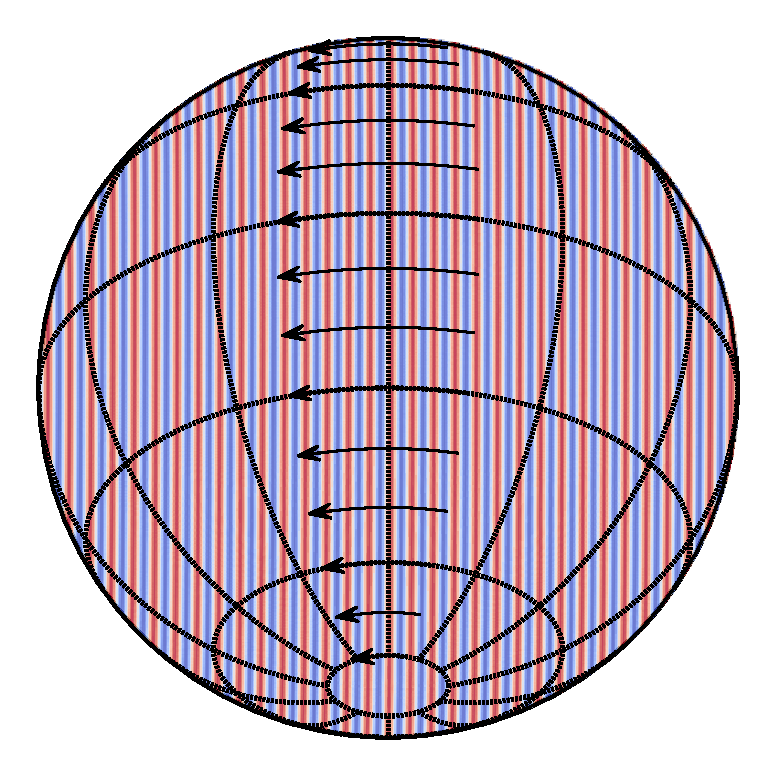
\includegraphics[width=.9\columnwidth]{plots/ew_fringe}
\caption{
The fringe pattern at 150 MHz of a 30-m east-west baseline, overlaid with arrows indicating
the distance traversed by sources at various declinations over a two-hour span centered at transit.
In a fixed time interval, sources near $\delta=0^\circ$ traverse more 
fringe periods than sources nearer to the celestial poles, giving rise to different
fringe rates that can be used to distinguish these sources in a timeseries measured with a single baseline.
}\label{fig:ew_fringe}
\end{figure}

\begin{figure}
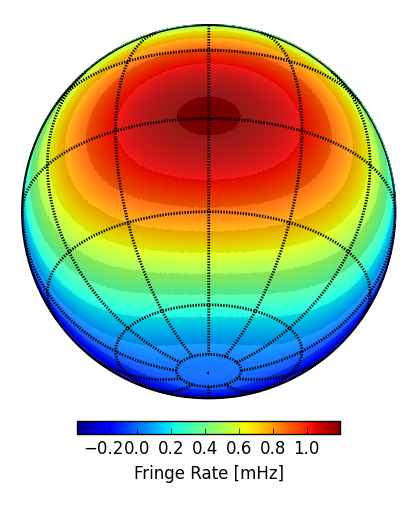
\includegraphics[width=.9\columnwidth]{plots/fringe_contours}
\caption{
Fringe rate as a function of sky position, corresponding to the fringe pattern illustrated in
Figure \ref{fig:ew_fringe}.  Fringe rates peak at XXX mHz at $\delta=0^\circ$, hit zero at
the south celestial pole, and become negative on the far side of the pole.  Grey shading indicates
the approximate angular regions that correspond to alternating fringe-rate bins, assuming a
fringe-rate transform taken over a two-hour time series.
}\label{fig:fringe_contours}
\end{figure}


\section{Fringe-rate filtering as mapmaking from time-ordered data}

Having provided some basic intuition for fringe-rate filtering, we now provide
a more formal treatment of the problem. In what follows, we will consider the
general problem of combining time-ordered visibilities into a map of the sky.
We will see that the optimal recipe for doing this is \emph{not} to time average
the visibilities, but instead, to apply a fringe-rate filter.

%[XXX: Say somewhere that unless otherwise stated, considering a drift-scan telescope.]
%[XXX: Don't forget to define hats as estimators, once and for all.]

%In this section, our goal is to examine how time-ordered visibilities from an
%interferometer should be best combined into information about the sky (such as
%an image-domain map).  Contrary to expectations, we will find that it is
%suboptimal to pursue the traditional, straightforward approach of averaging
%data in time, in the sense that such a procedure gives rise to
%larger-than-necessary error bars.  Instead, employing an unbiased,
%minimum-variance prescription naturally yields the technique of
%\emph{fringe-rate filtering}, the subject of this paper.

In this section, we re-motivate fringe-rate filters by
considering the problem of mapmaking from visibility data.  
Suppose our time-ordered visibilities are grouped into a measurement vector
$\vis$ of length $N_b N_t$, where $N_b$ is the number of baselines, and $N_t$
is the number of snapshots taken in time.  If we represent the true sky as a
vector $\x$ of length $N_\textrm{pix}$, and our instrument's response as a
matrix $\A$ of size $N_b N_t \times N_\textrm{pix}$, the measurement equation
is given by
\begin{equation}
\label{measEqn}
\vis = \A \x + \mathbf{n},
\end{equation}
where $\mathbf{n}$ is a noise vector.  Note that in this general form, Equation
\eqref{measEqn} is not basis-specific.  For example, while it is often useful
to think of $\x$ as a vector containing a list of temperatures in a set of
pixels on the sky (hence the variable name $N_\textrm{pix}$), it is equally
valid to employ another basis, such as spherical harmonics.  Similarly, while
we call $\vis$ the time-ordered data, it need not be a time series, and in
fact, a central message of this paper is that an optimal data analysis
prescription is more naturally phrased in terms of the Fourier dual to time,
i.e. fringe-rate.

Given our measurement $\vis$, the optimal estimator $\xhat$ of the true sky
$\x$ is given by \citep{Tegmark97,Morales2009} [XXX: add a citation to Josh
as well]
\begin{equation}
\label{optEst}
%\xhat = \left[ \A^\dagger \N^{-1} \A \right]^{-1} \A^\dagger \N^{-1} \vis,
\xhat = \mathbf{M} \A^\dagger \N^{-1} \vis,
\end{equation}
where $\mathbf{M}$ is some invertible matrix chosen by the data analyst, and
$\N$ is the noise covariance matrix, defined as $\langle \mathbf{n}
\mathbf{n}^\dagger \rangle$, with angled brackets denoting an ensemble average.
Again, our vector/matrix expressions are basis-independent, so even though the
formation of $\xhat$ is often described as ``mapmaking", it need not correspond
to spatial imaging in the traditional sense of the word.

The error bars on the estimator $\xhat$ are obtained by computing the square root
of the diagonal elements of the covariance $\boldsymbol \Sigma$, which is given by
\begin{equation}
\label{eq:sigma}
\boldsymbol \Sigma \equiv \langle (\x - \xhat) ( \x - \xhat)^\dagger \rangle = \mathbf{M} \A^\dagger \N^{-1} \A\mathbf{M}^\dagger.
\end{equation}
With a suitable choice of $\mathbf{M}$, the estimator given by Equation \eqref{optEst}
minimizes the variance. Regardless of one's choice, however, Equation \eqref{optEst} 
can be shown to be lossless \citep{Tegmark97}, in the sense that any quantities (such as power
spectra) formed further downstream in one's analysis will have identically
small error bars whether one forms these data products from $\xhat$ or chooses
to work with the larger and more cumbersome set of original data $\vis$.
%
%
%Regardless of the basis we work
%in, this estimator is unbiased, i.e.
%\begin{equation}
%\label{unbiased}
%\langle \xhat \rangle = \x,
%\end{equation}
%and has minimum variance, which is given by
%\begin{equation}
%\label{eq:sigma}
%\boldsymbol \Sigma \equiv \langle (\x - \xhat) ( \x - \xhat)^\dagger \rangle = \left[ \A^\dagger \N^{-1} \A \right]^{-1}.
%\end{equation}
%The estimator given by Equation \eqref{optEst} can also be proved to be
%lossless \citep{Tegmark97}, in the sense that any quantities (such as power
%spectra) formed further downstream in one's analysis will have identically
%small error bars whether one forms these data products from $\xhat$ or chooses
%to work with the larger and more cumbersome set of original data $\vis$.
%
%[XXX: add that the unbiased condition holds only when the matrix is invertible.]

In principle, Equation \eqref{optEst} is all that is needed to optimally
estimate the true sky.  One simply forms the relevant matrices and performs the
requisite matrix inversions and multiplications.  However, this is
computationally infeasible in practice, given that modern-day interferometers
are comprised of a large number of baselines operating over long integration
times, resulting in rather large matrices.  This is what motivated the authors
of \cite{Shaw2013} to propose their $m$-mode formalism, essentially rendering
many of the relevant matrices sparse, making them computationally easy to
manipulate.  While the $m$-mode formalism is a general framework that can be
used to solve a variety of problems (such as mitigating foreground
contamination), our goal here is to develop similarly convenient techniques for
the mapmaking problem (i.e., the formation of $\xhat$), with much detail
devoted to the intuition behind how our optimal estimator operates for an
interferometer.

\subsection{The general sub-optimality of time integration}
\label{timeSubOpt}

We begin by showing that it is suboptimal to make maps by integrating in time.
Consider the visibility response $V_b(t)$  of an interferometer baseline $b$ at
time $t$ to the sky $T(\rhat)$:
\begin{eqnarray}
\label{generalVis}
V_b(t) &&= \int B(\rhat, t) T(\rhat) \exp \left[ -i 2 \pi \left( \frac{b_y}{\lambda} \cos \eta \sin \delta \right) \right] \nonumber \\
&& \times  \exp \left[ -i 2 \pi \left( \frac{b_0}{\lambda} \cos \delta \sin(\alpha - \omega_\Earth t ) \right) \right]  d\Omega +n(t), \qquad
\end{eqnarray}
where $n(t)$ is the instrumental noise, $\alpha$ and $\delta$ are the right ascension and declination, respectively, $B(\rhat,t)$ is
the primary beam, $\lambda$ is the wavelength, $\omega_\Earth$ is the angular
frequency of the Earth's rotation, $\eta$ is the geographic latitude of the
array, and $b_0 \equiv \sqrt{b_x^2 + b_y^2 \sin^2 \eta}$, where $b_x$ and $b_y$
are the east-west and north-south baseline lengths, respectively.  We have chosen
our definition of $t=0$ to conveniently absorb an arbitrary constant phase. With this
measurement equation, we are assuming that the primary beam is fixed with
respect to local coordinates and translates azimuthally on the celestial
sphere.  We additionally assume that the baseline is phased to zenith.  In
other words, Equation \eqref{generalVis} describes an interferometer observing
in a drift-scan mode.

To see how integrating in time may be suboptimal, consider a simplified, purely
pedagogical thought experiment where our interferometer consists of a single
east-west baseline ($b_y=0$) situated at the equator ($\eta = 0$).  For the
primary beam, suppose we have a beam that is extremely narrow in the polar
direction, so that $B(\rhat, t) \equiv \delta^{(D)}(\delta)
B_\alpha(\alpha-\omega_\Earth t)$, where $ \delta^{(D)}$ signifies a Dirac delta
function.  Plugging these into restrictions into our
equation, we obtain
\begin{eqnarray}
\label{simpVis}
V_b (t) && = \int  \, B_\alpha(\alpha-\omega_\Earth t)  T \left( \delta = 0, \alpha \right) \nonumber \\
&&\times \exp \left[ -i 2 \pi  \frac{b_x}{\lambda} \sin(\alpha - \omega_\Earth t ) \right] d\alpha+ n(t).
\end{eqnarray}
For a single baseline, the function $V_b(t)$ is precisely the continuous version
of the discrete data vector $\vis$. To obtain $\vis$, then, one would simply sample
$V_b(t)$ discretely in time. For a multi-baseline array, forming $\vis$ involves following
the above procedure for each baseline, and then concatenating the resulting vectors
to form a single long $\vis$ vector. To make our analytic manipulations more convenient,
however, we will keep $t$ a continuous variable, so that $\vis$ is a hybrid quantity,
discrete in baseline but continuous in time. Acting on $\vis$ by a matrix then involves
summing over baselines and integrating over time.

Identifying $n(t)$ and $T(\theta= \pi / 2, \varphi)$ as
the continuous versions of $\mathbf{n}$ and $\x$ respectively, the rest of
Equation \eqref{simpVis}'s integrand can be interpreted as the continuous version of $\A$.  We
can model the noise covariance between baselines $b$ and $b^\prime$, at times
$t$ and $t^\prime$ as
\begin{equation}
\label{eq:noiseCovar}
N_{bb^\prime} (t, t^\prime) = \sigma^2 \delta_{bb^\prime} \delta(t-t^\prime),
\end{equation}
where $\sigma$ is an root-mean-square noise level assumed to be uncorrelated in
time and uncorrelated between baselines.

To see how the optimal prescription of Equation \eqref{optEst} combines
information from different times, we need only evaluate $\A^\dagger \N^{-1}
\vis$, for the $\mathbf{M}$ has no time index, so its application has no impact
on how time-ordered data is combined. In our toy model, we
have
\begin{equation}
\label{toyComb}
\left( \A^\dagger \N^{-1} \vis \right)_{\alpha} \! = \! \sum_b \!\!  \int \frac{dt}{\sigma^2} \,  B_\alpha(\alpha-\omega_\Earth t) \, e^{ i 2 \pi  \frac{b_x}{\lambda} \sin(\alpha - \omega_\Earth t ) } V_b(t),
\end{equation}
where the $\alpha$ variable serves as the continuous version of a discrete
vector index.  This expression shows that the optimal, minimum variance
prescription does not call for the integration of visibilities in time.
Instead, our expression calls for the \emph{convolution} of the visibility data
with a kernel that is specified by the primary beam shape and the baseline.

Now, recall from the convolution theorem that convolution in time is equivalent
to multiplication in the Fourier dual space of time.  For an interferometer
baseline, this Fourier dual space is fringe-rate.  Equation \eqref{toyComb}
therefore suggests that the optimal way to combine different time samples is to
express visibilities in fringe-rate space, and then to weight different
fringe-rates appropriately before summing.  We will develop this type of
fringe-rate filtering in full generality in Section \ref{fringeRateIntro},
demonstrating that its optimality is not a peculiarity of our current
pedagogical example, but is instead applicable in all situations.

%It is also important to emphasize that the technique of instantaneous
%snapshots---where one uses information from different baselines to form an
%instantaneous snapshot of the sky, which is then averaged with other snapshots
%to form a final image---is also sub-optimal.  In our notation, this would
%correspond to 

\subsection{The special case where integrating in time is optimal}

Before proceeding, it is instructive to establish the special case where time
integration is the optimal technique, since it is used so ubiquitously in the
literature.  An inspection of Equation \eqref{toyComb} shows that were it not
for the time-dependence in the primary beam and the time-dependence of the sky
moving through a baseline's fringes, the optimal recipe would indeed reduce to
an integration of visibilities in time.  Finding the limit where time
integration is optimal is then equivalent to finding a special case where the
aforementioned time-dependences vanish.

Recall that in our previous example, the primary beam had a time-dependence
only because our thought-experiment consisted of a drift-scan telescope, whose
measurement equation was written in coordinates fixed to the celestial sphere.
Instead of this, suppose one had a narrow primary beam that tracked a small
patch of the sky.  The primary beam would then have a fixed shape in celestial
coordinates, and $B(\rhat, t)$ would simply become $B(\rhat)$ in Equation
\eqref{generalVis}.  To attempt to nullify the time-dependence of fringes
sweeping across the celestial sphere, one may phase the visibilities in a
time-dependent way, essentially tracking the center of the patch as it moves
across the sky.  Putting this all together and assuming that the primary beam
is narrow enough to justify a flat-sky approximation, the measurement equation
becomes
\begin{eqnarray}
\label{flatSkyVis}
V_b(t) &&= \int B(\rhat) T(\rhat) \exp \left[ -i 2 \pi \left( \frac{b_0}{\lambda}  \sin(\alpha - \omega_\Earth t )\right) \right] \nonumber\\
&&\!\!\! \times \exp \left[-i 2 \pi \left( \frac{b_y}{\lambda} \cos \eta \cos \delta \right) + i \psi(t) \right] d\Omega +n(t), \qquad
\end{eqnarray}
[XXX: check this equation]
where we have assumed for simplicity that the center of our small field is
directly above the equator, and that a time-dependent phase $\psi(t)$ has been
applied.  With this, the optimal combination of time-ordered data becomes
\begin{eqnarray}
\left( \A^\dagger \N^{-1} \vis \right)_{(\delta,\alpha)}^\textrm{flat} &&  = \frac{B(\delta,\alpha)}{\sigma^2} e^{i 2 \pi \frac{b_y}{\lambda} \cos \eta \cos \delta}  \nonumber  \\
&&\!\!\! \times \sum_b \int  dt \,\,e^{ i 2 \pi  \frac{b_x}{\lambda} \sin(\alpha - \omega_\Earth t ) -i \psi (t) } V_b(t). \qquad
\end{eqnarray}
This is still not quite a simple average in time because there is no choice of
$\psi(t)$ that can cancel out the time-dependence of $\sin (\alpha -
\omega_\Earth t)$ for all $\varphi$ and all $t$.  Another way to phrase the
problem is to note that even in the flat-sky approximation, one cannot expand
Taylor expand $\sin (\alpha - \omega_\Earth t)$ over long observation times.
With short observations, however, an expansion is justified, and picking
$\psi(t) = 2 \pi \frac{b_x}{\lambda} \omega_\Earth t$ gives
\begin{eqnarray}
\left( \A^\dagger \N^{-1} \vis \right)_{(\theta,\varphi)}^\textrm{flat,short} =  &&\frac{B(\delta,\alpha)}{\sigma^2} e^{i 2 \pi \left( \frac{b_y}{\lambda} \cos \eta \cos \delta + \frac{b_x}{\lambda} \sin\alpha \right)} \nonumber \\
&& \times \sum_b   \int  dt \, V_b(t),
\end{eqnarray}
which is a simple averaging in time.  In short, then, integrating in time is an
optimal way to combine time-ordered data only if a number of criteria are met:
the flat-sky approximation must hold, the primary beam must track the field,
the visibilities must be phased to track the center of the field, and the
observations must be short.

[XXX: talk about how the same issues apply for a $uv$-plane description.]

[XXX: Maybe mention instantaneous snapshots and how it relates?]

[XXX: Fringe stopping at higher frequencies.]

\subsection{Fringe-rate filtering}
\label{fringeRateIntro}

We now proceed to derive the optimal prescription for combining time-ordered
data, which will lead us to the technique of fringe-rate filtering.  Because
our derivation will \emph{not} require any of the approximations that we have
invoked so far for pedagogical reasons, we will begin with our general
expression for time-ordered visibilities, Equation \eqref{generalVis}.  From
our toy example (Equation \ref{toyComb}), we know that fringe-rate space (the
Fourier dual of time) is a promising space in which to combine time-ordered
data.  Formally, measurements in this space are given by
\begin{equation}
\label{eq:FringeTransformDef}
\widetilde{V}_b (f) \equiv \frac{1}{T_\Earth} \int_{-T_\Earth / 2}^{T_\Earth /2} dt \exp \left( - 2 \pi i f t \right) V_b (t),
\end{equation}
where $f$ is the fringe-rate, and $T_\Earth = 2 \pi / \omega_\Earth$ is the
Earth's rotation period.  It is natural to work in fringe-rate bins such that
the $n^{th}$ bin is given by $f_n \equiv n / T_\Earth$, where $n$ is an
integer.  The measurement in the $n^{th}$ bin is then given by
\begin{eqnarray}
\label{fringeVis}
\widetilde{V}_b (f_n) &&= \int d\Omega \, T(\rhat) e^{-i 2 \pi  \frac{b_y}{\lambda} \cos \eta \sin \delta} \nonumber \\
&& \!\!\!\times  \int_{-\frac{T_\Earth}{ 2}}^{\frac{T_\Earth}{2}} \frac{dt}{T_\Earth} \, B(\rhat, t) e^{ -i  \frac{2 \pi n t}{T_\Earth} +i  \frac{2\pi b_0}{\lambda} \cos \delta \sin \left( \omega_\Earth t - \alpha \right)}, \qquad
\end{eqnarray}
where we have temporarily omitted the additive noise term to avoid mathematical
clutter.  To proceed, we make some simplifying assumptions (although only some
of which are absolutely required).  First, assume that we are once again
considering a drift-scan instrument.  If the primary beam shape is
approximately separable, we can then say
\begin{equation}
\label{eq:SepBeam}
B(\rhat, t) \equiv B_\delta (\delta) B_\alpha (\alpha - \omega_\Earth t),
\end{equation}
where $B_\alpha$ is a function with period $2\pi$.  Taking advantage of this periodicity, we can write the beam as
\begin{equation}
B(\rhat, t) = B_\delta (\delta) \sum_q \widetilde{B}_q e^{-iq \alpha} e^{i q \omega_\Earth t},
\end{equation}
where $\widetilde{B}_q \equiv \int \frac{d\alpha}{2\pi} B_\alpha(\alpha)
e^{i q\alpha}$ is the $q^{th}$ Fourier coefficient.  Plugging this into
Equation \eqref{fringeVis} and making the substitution $\psi \equiv
\omega_\Earth t - \varphi$, one obtains
\begin{eqnarray}
\widetilde{V}_b (f_n) &&= \int d\Omega \, T(\rhat) B_\delta (\delta) e^{-i 2 \pi  \frac{b_y}{\lambda} \cos \eta \sin \delta} \nonumber \\
&& \times \sum_q \frac{\widetilde{B}_q e^{-i n \varphi}}{2 \pi} \int_{-\pi -\varphi}^{\pi+\varphi} d\psi \, e^{i (q-n) \psi +i \frac{2 \pi b_0}{\lambda} \cos \delta \sin \psi}. \qquad
\end{eqnarray}
Now, note that the integral over $\psi$ is of a periodic function over one
period.  We may therefore freely shift the limits of the integral by a constant
amount without affecting the result.  In particular, we may remove the
$+\varphi$ terms in the limits (the only restriction being that having performed a $\varphi$-dependent shift, it is no longer legal to permute the various integrals), and
the result is a standard integral form for a Bessel function $J$ of the first
kind:
\begin{eqnarray}
\label{fringeBessel}
\widetilde{V}_b (f_n) =&& \int \frac{d\Omega}{2 \pi}\, T(\rhat) B_\delta (\delta) e^{-i 2 \pi  \frac{b_y}{\lambda} \cos \eta \sin \delta}
e^{-i n \alpha} \nonumber \\ 
&& \times \sum_q \widetilde{B}_q  J_{n-q} \left( \frac{2 \pi b_0}{\lambda} \cos \delta \right).
\end{eqnarray}
Several features are of note here.  For wide primary beams, $\widetilde{B}_q$
is sharply peaked around $q=0$, so the terms following the sum over $q$
essentially amount to $J_n ( 2 \pi b_0 \cos \delta / \lambda )$.  Now, notice
that the argument of the Bessel function is bounded, always lying between $\pm
2\pi b_0/ \lambda$.  For large $n$ (high fringe-rate bins), then, one can use
the small argument asymptotic form for $J_n$,\begin{equation}
J_n \left( \frac{2 \pi b_0 \cos \delta}{ \lambda} \right) \approx \frac{1}{n!} \left( \frac{ \pi b_0 \cos \delta}{ \lambda} \right)^n,
\end{equation}
which is a sharply decreasing function of $n$ for large $n$.  This means that
there must be very little sky signal at high fringe-rate bins.  Intuitively,
this is because sources on the celestial sphere have their fringe rates limited
by the Earth's rotation period and projected baseline length $b_0$, making high
fringe rates physically unattainable by true celestial emission.  Any signals
seen in high fringe-rate bins will therefore be primarily due to noise.

With celestial emission appearing only in low fringe-rate bins, it is
reasonable to expect that one can reduce noise (in other words, achieving the
goals of time integration) by Fourier transforming the data into fringe-rate
space and downweighting (or discarding) high fringe-rate modes.  This is
confirmed by constructing the optimal prescription as we did above, which
yields
\begin{eqnarray}
\label{eq:AdagNinvv}
\left( \A^\dagger \N^{-1} \vis \right)_{\delta,\alpha} && = \frac{B_\delta^* (\delta)  \cos \delta}{2\pi \sigma^2} \sum_{b,n} e^{i n \alpha} e^{i 2 \pi  \frac{b_y}{\lambda} \cos \eta \sin \delta} \nonumber \\
&& \times \sum_{q} \widetilde{B}_q^* J_{n-q} \left( \frac{2 \pi b_0}{\lambda} \cos \delta \right) \widetilde{V}_b (f_n).
\end{eqnarray}
In words, this recipe instructs us to move into fringe-rate space (where the
sky emission is already concentrated in $f_n$) and to further downweight by
$\sum_{q} \widetilde{B}_q^* J_{n-q} \left( \frac{2 \pi b_0}{\lambda} \cos \delta \right)$, which, as we have argued above, is small for high fringe
rates.  Thus, low-pass fringe-rate filtering is the optimal way to combine
time-ordered data from an interferometer.

Before proceeding, let us summarize the essential features of fringe-rate filtering, away from the approximation of a separable beam in Equation \eqref{eq:SepBeam}. Returning to Equations \eqref{eq:FringeTransformDef} and \eqref{fringeVis}, we see that because the sky $T(\hat{\mathbf{r}})$ is not a function of time, the Fourier transform into fringe-rate space acts only on the beam and the fringe pattern. We can therefore write
\begin{equation}
\label{eq:CompactNotation}
\widetilde{V}_b (f_n) = \int d\Omega \,T(\hat{\mathbf{r}}) g_{bn} (\hat{\mathbf{r}}) 
%\approx \frac{4 \pi}{N}  \sum_i T(\hat{\mathbf{r}}_i) g_{bn} (\hat{\mathbf{r}}_i)
,
\end{equation}
where the key quantity is
\begin{eqnarray}
g_{bn} (\hat{\mathbf{r}})  &&\equiv e^{-i 2 \pi  \frac{b_y}{\lambda} \cos \eta \sin \delta} \nonumber \\
 &&\times \int_{-\frac{T_\Earth}{ 2}}^{\frac{T_\Earth}{2}} \frac{dt}{T_\Earth} \, B(\rhat, t) e^{ -i  \frac{2 \pi n t}{T_\Earth} +i  \frac{2\pi b_0}{\lambda} \cos \delta \sin \left( \omega_\Earth t - \alpha \right)}. \qquad
\end{eqnarray}
The term in front of the integral corresponds to the fringes in the declination direction. These are static as the Earth rotates, and therefore are unaffected by the Fourier transform. The second half of the exponent within the integral corresponds to fringes in the azimuthal direction, with the $\cos \delta$ term arising because of the spherical geometry shown in Figure \ref{fig:ew_fringe}, where sources near the equator traverse fringes more quickly than those near the pole. Examining the integral, we see that there are two contributions to a non-zero fringe-rate. First, the primary beam sweeps across the celestial sphere, crossing fringes. In addition, the changing orientation of baselines relative to the celestial sphere induces a fringe-rate. Over a short time-integration (which is likely a more realistic scenario than integrating over $T_\Earth$ as we have assumed so far) we may approximate this second contribution by Taylor expanding the $\sin(\omega_\Earth t - \alpha)$ term. This yields a time-dependence that may be absorbed into the $\exp \left(-i 2 \pi n t / T_\Earth \right)$ term as an additive term to the fringe-rate bin $n$. What remains is then simply a phase-shifted Fourier transform of the primary beam. In other words, $g_{bn} (\hat{\mathbf{r}})$ selects portions of the primary beam where sources on the sky have a fringe-rate of $n/ T_\Earth$. Now, since
$\widetilde{V}_b (f_n)  = \int d\Omega  \,T (\hat{\mathbf{r}}) g_{bn} (\hat{\mathbf{r}})$, each row of the matrix $\mathbf{A}$ corresponds to $g_{bn} (\hat{\mathbf{r}})$ for a different baseline $b$ and/or fringe rate bin $n$, and our optimal prescription for combining time-ordered data becomes
\begin{equation}
\left( \A^\dagger \N^{-1} \vis \right)_{\delta,\alpha} \propto \sum_{n,b} g_{bn}^* (\hat{\mathbf{r}}) \widetilde{V}_b (f_n).
\end{equation}
One sees that the procedure essentially calls for a weighting that emphasizes the fringe rate bins that fall on bright portions of the primary beam. As seen in our toy example, this preferentially favors lower fringe-rates over higher ones.
%
%\section{Mapping fringe-rates to spatial locations over short integration times}
%
%In the previous section, we considered a general way to combine time-ordered interferometric data, and found that fringe-rate filtering provided a natural way to do so. In this section, we provide an approximate treatment of the more realistic case where one cannot integrate over an entire day. The result will provide a rigorous link to the geometric intuition discussed in Section \ref{sec:overview}.
%
%\begin{equation}
%V_b(t) = \int d\Omega B (\rhat,t) T(\rhat) \exp\left( i \frac{2 \pi }{\lambda} \mathbf{b} (t) \cdot \rhat \right)
%\end{equation}
%\begin{equation}
%\widetilde{V}_b (f) = \int d\Omega T(\rhat) \int_{-\frac{T}{2}}^{\frac{T}{2}} \frac{dt}{T} B (\rhat,t) e^{i \frac{2 \pi }{\lambda} \mathbf{b} (t) \cdot \rhat } e^{-i 2 \pi f t}
%\end{equation}
%For short periods of time, $B (\rhat,t) \approx B (\rhat,t=0) \equiv B_0 (\rhat)$. Also,
%\begin{equation}
%\mathbf{b}(t) = \mathbf{b}(t=0) + \frac{d\mathbf{b}}{dt} \Bigg{|}_{t=0} t + \dots = \mathbf{b}_0 + (\boldsymbol \omega_\Earth \times \mathbf{b}_0) t + \dots
%\end{equation}
%where $\boldsymbol \omega_\Earth$ is the angular velocity vector of the Earth's rotation, and $\mathbf{b}_0 \equiv \mathbf{b}(t)$. In the last equality, we used the fact that the time-dependence of the baselines are not arbitrary, but instead are tied to the Earth's rotation, transforming the time derivative into a cross-product with $\boldsymbol \omega_\Earth$. With this,
%\begin{eqnarray}
%\widetilde{V}_b (f) = &&\int d\Omega T(\rhat) B_0 (\rhat)  e^{i \frac{2 \pi }{\lambda} \mathbf{b}_0 \cdot \rhat } \nonumber \\
%&&\times \int_{-\frac{T}{2}}^{\frac{T}{2}} \frac{dt}{T} \exp\left[i \frac{2 \pi }{\lambda}  \rhat \cdot (\boldsymbol \omega_\Earth \times \mathbf{b}_0) t-i 2 \pi f t \right] \nonumber \\
%= && \int d\Omega T(\rhat) B_0 (\rhat)  \textrm{sinc} \left[ \pi T \left( \rhat \cdot \boldsymbol \omega_\Earth \times \frac{\mathbf{b}_0}{\lambda} -f \right) \right] e^{i \frac{2 \pi }{\lambda} \mathbf{b}_0 \cdot \rhat }.
%\end{eqnarray}
%The sinc function is peaked near zero argument, and thus its presence in the integral enforces that $f \approx \rhat \cdot \boldsymbol \omega_\Earth \times \mathbf{b}_0 / \lambda $, picking out only specific portions of the celestial sphere. As advertised, different fringe-rates correspond to different portions of the sky.
%
%Fringe-rate filtering amounts to decomposing into the fringe-rates, weighting fringe rates by some function $w(f)$, and then transforming back to time. In other words,
%\begin{equation}
%V_\textrm{filt} (t) = \int \frac{df}{1/T} w(f) \widetilde{V}_b (f) 
%\end{equation}
%
%\section{Combining time-ordered data without mapmaking}
%
%Until now, our discussion of fringe-rate filtering has centered around the mapmaking problem.  However, our intuitive understanding of fringe-rate filtering---that it differentiates instrumental noise from celestial signals by identifying high fringe-rates as being noise-dominated---holds much more generally.    In this section, we show how fringe-rate filtering can be used a de-noising tool for visibilities, bypassing the image domain entirely.  This allows one to take advantage an important benefit of mapmaking, namely, the reduction of instrumental noise through the coherent combination of time-ordered data, while avoiding some of its drawbacks such as the introduction of curved-sky or gridding artifacts.  Moreover, for many applications (such as power spectrum estimation), it is more natural to work with interferometric visibilities directly, provided they can be de-noised.
%
%To de-noise our visibilities, suppose (for a brief moment) that one did in fact produce an estimator $\xhat$ of the sky in the image domain.  One could then transform this estimator back into time-ordered visibilities $\vis_\textrm{filt}$ by simply computing $\vis_\textrm{filt} \equiv \A \xhat$.  Such a set of visibilities would represent de-noised visibilities since Equation \eqref{optEst} is essentially a best-fit solution based on noisy data, which means that $\A \xhat$ is simply the set of predicted visibility measurements from the best-fit model.  Now, if these predicted measurements were actually generated by first forming a map, one would still incur all the difficulties in imaging that one had hoped to avoid.  To deal with this issue, we note that the relationship between the original visibilities and the de-noised ones are given by
%\begin{equation}
%\label{eq:filt}
%\vis_\textrm{filt} = \A \mathbf{M} \A^\dagger \N^{-1} \vis \equiv \mathbf{W}  \vis.
%\end{equation}
%The matrix $\mathbf{W}$ can be thought of as a de-noising filter, and if it can be computed analytically we will have bypassed imaging entirely.
%
%As we discussed in the previous section, our fringe-rate filtering preferentially downweights higher fringe-rate modes. In doing so, care must be taken to ensure that the resulting data are normalized correctly. This is synonymous with normalizing $\mathbf{M}$ correctly. One choice would be $\mathbf{M} = \left[ \A \N^{-1} \A \right]^{-1}$. By combining Equations \eqref{measEqn} and \eqref{optEst}, one sees that such a choice yields $\langle \hat{\mathbf{x}} \rangle = \mathbf{x}$, which is not only correctly normalized, but also has all point spread function effects removed from images. Unfortunately, the combination $\A \N^{-1} \A$ is not always invertible, precisely because it is in general impossible to perfectly remove the effects of a telescope's point spread function. However, we can still obtain a normalized estimator of the sky by picking $\mathbf{M}_{ij} = \left[ \A \N^{-1} \A \right]_{ii}^{-1} \delta_{ij}$. The resulting point spread function is peak-normalized to unity.
%
%Consider first a single baseline. Reading off the discretized version of Equation \eqref{eq:CompactNotation}, we can relate $\A$ to $g_{bn} (\mathbf{\hat{r}})$. Assuming again that
%$\N \propto \mathbf{I}$, a little algebra reveals that
%\begin{equation}
%\mathbf{W}_{ij} = \sum_m \frac{g_{bi }(\mathbf{\hat{r}}_m) g_{bj }^*(\mathbf{\hat{r}}_m)}{\sum_j | g_{bj} (\mathbf{\hat{r}}_m) |^2}.
%\end{equation}
%As per Equation \eqref{eq:filt}, this is a matrix operator that is applied to the original visibilities to give the filtered ones. Rather than applying a full matrix operator, some of the same effects can be achieved with just a diagonal approximation, i.e., by simply weighting with some scalar weights. Defining the $i$th weight $w_i$ to be $\mathbf{W}_{ii}$, we have
%\begin{equation}
%w_i = \sum_m \frac{| g_{bi} (\mathbf{\hat{r}}_m) |^2}{\sum_j | g_{bj} (\mathbf{\hat{r}}_m) |^2}.
%\end{equation}
%One sees from this that the fringe rates that do not have a strong presence in the primary beam (in the sense of the geometric mapping between fringe rates and locations of the sky illustrated in Figure \ref{fig:fringe_contours}) are downweighted. XXX: Not sure why the normalization is coming out to the number of pixels.

\section{Power Spectrum Estimation with Fringe-Rate Filtering}
\label{sec:OptPower}
We now discuss the problem of power spectrum estimation given time-ordered data.  The primary challenge, again, is to ensure that the benefits of a long time-integration (i.e. increased sensitivity) can be realized without explicitly making maps.  For example, one cannot simply average over power spectrum estimates formed from every time instant of some time-ordered visibilities.  Doing so would reduce the sensitivity of the final power spectrum, as coherent information between time-samples would be lost.  However, it would be desirable to be able to optimally include coherent information while remaining in a time-ordered basis where systematic effects are transparent.  In this section, we will show that the techniques of fringe-rate filtering make it possible to construct a power spectrum estimator that satisfies these requirements.

We start with the estimator $\hat{p}_\alpha$ for the $\alpha$th band of the power spectrum:
\begin{equation}
\label{eq:GenFormPowEst}
\hat{p}_\alpha = N_\alpha \hat{\x}^\dagger \mathbf{C}^{-1} \mathbf{Q}_\alpha \mathbf{C}^{-1} \hat{\x},
\end{equation}
where $\mathbf{C} \equiv \langle \hat{\x} \hat{\x}^\dagger \rangle = \mathbf{S} + \boldsymbol \Sigma$ is the \emph{total} (signal plus noise) covariance matrix of the sky map, and $N_\alpha$ is a normalization factor, given by\footnote{More sophisticated normalization schemes involving matrix normalization constants are possible [XXX: cite Josh MWA paper], but for simplicity (and no loss of generality as far as our present discussion is concerned) we do not consider them here.}
\begin{equation}
N_\alpha = \textrm{tr} \left[ \mathbf{C}^{-1} \mathbf{Q}_\alpha \mathbf{C}^{-1} \mathbf{Q}_\alpha \right].
\end{equation}
[XXX: grr...the Fisher matrix isn't diagonal here, so it's a little more annoying when it comes to normalization.  Need to decide which norm convention to use].  Written in this general form, our estimator can be used to estimate any power spectrum, be it an angular power spectrum $C_\ell$ (in which case $\hat{p}_\alpha \equiv \hat{C}_\ell$ and $\alpha$ would index the $\ell$ value), or a three-dimensional power spectrum $P(\mathbf{k} )$ (in which case $\hat{p}_\alpha \equiv \hat{P}(\mathbf{k}_\alpha)$).  The type of power spectrum under consideration is encoded by the form of the $\mathbf{Q}_\alpha$ matrices.  They are defined as the linear response of the covariance matrix $\mathbf{C}$ to the power spectrum:
\begin{equation}
\mathbf{Q}_\alpha \equiv \frac{\partial \mathbf{C}}{\partial p_\alpha}.
\end{equation}
The inverse-covariance weighting enacted by $\mathbf{C}^{-1}$ makes Equation \eqref{eq:GenFormPowEst} a minimum-variance estimator \citep{liu_tegmark2011}.  For notational cleanliness we have omitted any corrections to \emph{additive} biases in the estimator, implicitly assuming that such biases have already been removed.

As it stands, our estimator is written explicitly in terms of the estimated sky maps $\hat{\x}$.  These are related to the visibilities via Equation \eqref{optEst}, which states that $\xhat = \left[ \A^\dagger \N^{-1} \A \right]^{-1} \A^\dagger \N^{-1} \vis$.  If we assume that our measurements are noise-dominated, then $\mathbf{C} \approx \boldsymbol \Sigma = [ \mathbf{A}^\dagger \mathbf{N}^{-1} \mathbf{A} ]^{-1}$, so $\mathbf{C}^{-1} \approx [ \mathbf{A}^\dagger \mathbf{N}^{-1} \mathbf{A} ]$.  Inserting these into Equation \eqref{eq:GenFormPowEst}, we obtain
\begin{equation}
\label{eq:VisBasedPowEst}
\hat{p}_\alpha = N_\alpha \hat{\vis}^\dagger \N^{-1} \A  \mathbf{Q}_\alpha \A^\dagger \N^{-1} \vis
\end{equation}
as our visibility-based estimator.

To see how fringe-rate filters relate to this expression, consider the specific example of measuring the angular power spectrum $C_\ell$.  In this case, we parameterize the signal covariance in terms of spherical harmonics, so that
\begin{equation}
\mathbf{C}_{\hat{\r}, \hat{\r}^\prime} = [ \mathbf{A}^\dagger \mathbf{N}^{-1} \mathbf{A} ]^{-1} + \sum_{\ell m} Y_{\ell m} ( \hat{\r}) Y^*_{\ell m} (\hat{\r}^\prime) C_\ell,
\end{equation}
and thus
\begin{equation}
\label{eq:CEllQ}
\mathbf{Q}_\ell \equiv \frac{\partial \mathbf{C}}{\partial C_\ell} = \sum_{m} Y_{\ell m} ( \hat{\r}) Y^*_{\ell m} (\hat{\r}^\prime),
\end{equation}
where we have renamed the index $\alpha$ to $\ell$ as a reminder that we are considering the angular power spectrum.  Note that since the noise covariance does not depend on the power spectrum $C_\ell$, it is necessary to include the signal covariance when deriving $\mathbf{Q}_\ell$, even though this was unnecessary for $\mathbf{C}^{-1}$.

Substituting Equations \eqref{eq:AdagNinvv} and \eqref{eq:CEllQ} into Equation \eqref{eq:VisBasedPowEst}, we obtain
\begin{equation}
\label{eq:StillFringe}
\widehat{C}_\ell \propto \sum _{m=-\infty}^\infty \Bigg{|} \sum_b w_{\ell m}^b \widetilde{V}_b (f_m) \Bigg{|}^2,
\end{equation}
where
\begin{equation}
w_{\ell m}^b \equiv
\begin{cases}
2 \pi \int d(\cos \theta) N_{\ell}^m P_{\ell}^{m} (\cos \theta) g_b(\theta,m),& \textrm{for} -\ell \leq m \leq \ell \\
0, & \textrm{otherwise,}
\end{cases}
\end{equation}
with $P_\ell^m$ being the associated Legendre polynomial of order [XXX: insert proper name here], and
\begin{equation}
N_\ell^m = \sqrt{\frac{2\ell + 1}{4 \pi} \frac{(\ell-m)!}{(\ell + m )!}}
\end{equation}
is the normalization constant for spherical harmonics.  Since we can equivalently interpret $m$ not as the azimuthal Fourier mode number but as the fringe-rate bin index, it is the Fourier dual to time, our estimator can be rewritten using Parseval's theorem:
\begin{equation}
\label{eq:FinalTimeEst}
\widehat{C}_\ell \propto  \int_{-T_\Earth / 2}^{T_\Earth /2} \frac{dt}{T_\Earth} \Bigg{|} \sum_b V^\textrm{filt}_{\ell b} (t) \Bigg{|}^2,
\end{equation}
where
\begin{equation}
\label{eq:FinalFilt}
V^\textrm{filt}_{\ell b} (t) \equiv  \sum_m \exp \left[i \frac{2 \pi m t}{T_\Earth}\right]  w_{\ell m}^b \widetilde{V}_b (f_m).
\end{equation}
Together, Equations \ref{eq:FinalTimeEst} and \ref{eq:FinalFilt} suggest a method for estimating power spectra.  First, time-ordered visibilities are Fourier-transformed into a fringe-rate basis.  Different fringe-rate bins are then weighted by the $w_{\ell m}^b$ weights, which essentially encode the ``dot product" between a baseline's response in the fringe-rate bin and the angular mode in question.  The result is then transformed back into a set of fringe-rate filtered visibility time series.  A power spectrum is computed for every time instant before averaging together different times.  Since this procedure was derived from a minimum-variance estimator of the power spectrum, it is guaranteed to produce the smallest possible error bars.

We have thus accomplished our goal of writing down an optimal estimator for the power spectrum that works directly with visibilities.  Conveniently, the integration of coherent information takes place via a fringe-rate filter, which operates on independently for different baselines.  Moreover, since it returns data in its original format---a time-series---systematics localized to certain baselines and certain times can be easily isolated.  Note that while the filtering is performed per-baseline, information from multiple baselines regarding the same $\ell$ mode is coherently included before squaring to form the power spectrum.  This is most clearly seen in Equation \eqref{eq:StillFringe}, where visibilities from different baselines are simply added together, except that they are weighted by different amounts depending on how much overlap they have with the mode in question.  Traditionally, taking advantage of coherent information between non-identical baselines requires imaging (whether in the image basis or as a Fourier-transformed image in the form of, say, $uv$-plane data).  With our approach, imaging (and its attendant artifacts) are completely avoided without sacrificing sensitivity.
[XXX: JUST REALIZED THIS IS FAR MORE ALGORITHMICALLY EFFICIENT THAN MAPMAKING!!!]

[XXX: Maybe also consider $l \sim 2 \pi b / \lambda$ approx.]
[XXX: Perhaps make connection to thingy more clear.]
[XXX: Consider also playing up the weights as the ``dot product" of the thing you're interested in and the fringe-rate-space visibilities to emphasize how different baselines just need to combined based on their overlap.]
%
%One approach to forming an estimate of the power spectrum would be to start from the Wiener-filtered visibilities from the previous section.  As mentioned above, however, doing so would result in a power spectrum that contained a multiplicative bias.  A straightforward fix to this problem would be to appropriately normalize the Wiener weights derived in Equation \eqref{eq:WienerWeights}.  Roughly speaking, those fringe-rates that were biased low by the Wiener filter can simply be renormalized to the appropriate level.  We caution, however, that this renormalization cannot be done on a fringe-rate-by-fringe-rate basis, since the diagonal nature of $\mathbf{W}^\textrm{Wiener}$ would result in the identity matrix.  (This follows immediately from the arguments that led us to impose a prior on the signal covariance matrix, namely that each fringe-rate bin probes unique information on the sky).  However, a typical power spectrum estimator takes advantage of statistical isotropy to sum together the power estimates of individual azimuthal modes (or equivalently, fringe rates).  To arrive at a power-conserving normalization, then, we simply require that the summed power estimates are properly normalized.  This allows different fringe rates to retain their relative normalization, preserving the de-noising ability of our filter.   [	XXX: should we explicitly construct the sub-optimal Wiener-filter-based estimator?]
%
%While the aforementioned procedure will indeed result in an unbiased power spectrum estimator, 
%
%Before deriving the correct normalization factors, we first pause to discuss the optimality of this procedure.   At first glance, the normalized Wiener-filter that we just described is not guaranteed to be an optimal way to estimate the power spectrum (in the sense of producing minimum-variance power spectrum estimates), since the Wiener filter was constructed only to minimize errors in images.  We will now show, however, that in the low signal-to-noise regime discussed above, the procedure is in fact optimal, and is derivable from an optimal power spectrum estimator.  We start with the estimator $\hat{p}_\alpha$ for $P(k_\alpha)$:
%\begin{equation}
%\hat{p}_\alpha = N_\alpha \hat{\x}^\dagger \mathbf{C}^{-1} \mathbf{Q}_\alpha \mathbf{C}^{-1} \hat{\x},
%\end{equation}
%where $\mathbf{C} \equiv \langle \hat{\x} \hat{\x}^\dagger \rangle = \mathbf{S} + \boldsymbol \Sigma$ is the \emph{total} (signal plus noise) covariance matrix of the sky map, and $N_\alpha$ is a normalization factor.  The inverse-covariance weighting enacted by $\mathbf{C}^{-1}$ makes this a minimum-variance estimator \citep{liu_tegmark2011}, and for notational cleanliness we have omitted any corrections to \emph{additive} biases in the estimator, implicitly assuming that such biases have already been removed.  \cite{seljak1998} showed that this estimator can easily rewritten in terms of the Wiener-filtered estimator for the sky:
%\begin{eqnarray}
%\label{eq:WienerPowerEst}
%\hat{p}_\alpha &=& N_\alpha \hat{\x}^\dagger_\textrm{Wiener} \mathbf{S}^{-1} \mathbf{Q}_\alpha \mathbf{S}^{-1} \hat{\x}_\textrm{Wiener} \nonumber \\
%&=& N_\alpha \hat{\x}^\dagger_\textrm{Wiener}  \mathbf{Q}_\alpha \hat{\x}_\textrm{Wiener},
%\end{eqnarray}
%where in the second equality we assumed, like before, that $\mathbf{S} = \sigma_s^2 \mathbf{I}$ and absorbed the $\sigma_s^2$ into the normalization.  As it currently stands, the power spectrum estimator takes maps (whether Wiener filtered or not) as input.  In a similar spirit to the previous section, we would prefer to evade imaging artifacts by working directly from visibilities.  To rewrite Equation \eqref{eq:WienerPowerEst}, we make use of the following trick.  Working from Equation \eqref{manifest}, it is clear that
%\begin{equation}
%(\mathbf{A}^\dagger \mathbf{A} )_{m, \theta ; m^\prime \theta^\prime} = \delta_{mm^\prime} g_b(\theta, m) g_b^*(\theta^\prime, m^\prime).
%\end{equation}
%Suppose we apply this operator to $\hat{\x}_\textrm{Wiener}$ (the motivation for this will become clear momentarily), which we can express as 
%\begin{equation}
%\xhat_\textrm{Wiener} = \frac{\sigma_s^2}{\sigma_n^2} \mathbf{A}^\dagger  \vis,
%\end{equation}
%
%
%This process---first Wiener-filtering and then 
%
%[XXX: Discuss the assumptions made.]
%
%As an example, suppose one were to form an estimator of the angular cross-power spectrum $C_\ell$ between the sky at two frequencies:
%\begin{equation}
%\label{eq:C_Ell}
%\widehat{C}_\ell (\nu, \nu^\prime) \propto \frac{1}{2\ell + 1} \sum_{m=-\ell}^{\ell} \vis^*_m (\nu) \vis_m (\nu^\prime),
%\end{equation}
%where $K=...$ [XXX: put in a conversion factor for Jy to K etc. Need to be better about the distinction between xhat and v].  If one makes the assumption that a given baseline's response is strongly peaked at the specific angular mode $\ell \sim 2 \pi \sqrt{b_x^2+ b_y^2} / \lambda$, we will only need to consider the estimator on a baseline-by-baseline basis.  If the input visibilities are chosen to be the Wiener-filtered ones, this estimator can be shown to be an optimal, minimum-variance estimator [XXX: need to dig up Ue-Li and Uros' paper references].  Now, isotropy dictates that all azimuthal Fourier modes contribute the same power.  To ensure that the power spectrum estimate is properly normalized, we therefore require the \emph{square} of the weights given by Equation \eqref{eq:WienerWeights} sum to unity.  In other words, for the purposes of power spectrum estimation one weights the $n^\textrm{th}$ fringe-rate bin by
%\begin{equation}
%w_n = \frac{ \int_0^{\pi}  | g_b (\theta, n) |^2 d\theta}{\sum_m \left( \int_0^{\pi}  | g_b (\theta^\prime, m) |^2 d\theta^\prime \right)^2 },
%\end{equation}
%with filtered visibilities given by $v^\textrm{filt}_n = w_n v_n$.
%
%Equation \eqref{eq:C_Ell} can be written in terms of a time-series by the nothing the following.  Since the interferometer response decays rapidly for large fringe-rate bins, we can extend the sum over $m$ to go from $-\infty$ to $+\infty$.  Then recalling that $m$ doubles as the fringe-rate index, which is the Fourier dual to time, one can use Parseval's theorem to write
%\begin{equation}
%\widehat{C}_\ell \propto \frac{1}{2\ell +1}  \int_{-\frac{T_\Earth}{2}}^{\frac{T_\Earth}{2}} \frac{dt}{T_\Earth}   V_{\textrm{filt}}^* (\nu,t) V_\textrm{filt} (\nu^\prime,t),
%\end{equation}
%where
%\begin{equation}
%V_\textrm{filt}(\nu,t)=  \sum_m \exp \left[i \frac{2 \pi m t}{T_\Earth}\right] w_m v_m (\nu).
%\end{equation}
%Written in this way, it is clear that the optimal power spectrum estimator reduces to averaging together estimators that are formed at every instant in time---provided that one uses the fringe-rate filtered visibilities instead of the original, unprocessed visibilities.  Ordinarily, forming power spectra at every instant is suboptimal because it involves the squaring of visibilities, resulting in the loss of coherent phase information.  In other words, one cannot coherently add together constraints on the same sky information from different time slices, and errors in the power spectrum average down as $1/\sqrt{t}$.  Traditionally, coherent integration is implemented by first forming a map of the sky (in whatever basis one desires), and then to estimate the power spectrum from the maps.  The final errors on the power spectrum then decrease as $1/t$.  What has been shown here is that fringe-rate filtered visibilities are visibilities that have effectively already been coherently integrated in time, and estimating the power spectrum time-slice-by-time-slice with them represents no loss of sensitivity.  Working in a time basis can be preferable to using Equation \eqref{eq:C_Ell} directly because many systematics can be more easily isolated by examining time-series data.  Our analytic expressions allow fringe-rate filtering to be performed without mapmaking, reducing the possibility of image-domain artifacts and curved-sky complications.
%
[XXX: Need to find a place to talk about effective beams and how it affects power spectrum sensitivity.  Talk about how we will henceforth use simulated effective beams so that we don't have to make all the assumptions that went into the analytic work.  Should also credit Richard for the fringe-rate --> m-mode correspondence more throughout.]


%While we established in the previous section that Wiener-filtered visibilities would give biased estimates of the power spectrum, we can fortunately sidestep the problem by making a different assumption---that of isotropy.
%
%To pick a concrete example that will serve as the focus for the rest of the paper, consider the power spectrum $P(\mathbf{k})$ of highly redshifted $21\,\textrm{cm}$ emission.  At each instant, spatial fluctuations that are perpendicular to the line-of-sight are probed by the fringe-patterns of a baseline, while the spectral nature of the measurement means that structure along the line-of-sight is accessed by the frequency spectrum of the visibilities.  Specifically, if one performs a delay transform on a baseline's visibility by Fourier transforming its frequency spectrum (thus expressing the spectrum in delay space), the result is a probe of the Fourier mode with wavevector $\mathbf{k} \approx 2 \pi (b_x / \lambda X, b_y / \lambda X, \tau /Y)$, where $b_x$ and $b_y$ are the x- and y-components of the baseline vector, respectively, $\tau$ is the delay.  The scalars $X$ and $Y$ convert angles and frequency to comoving distances, respectively.  In the limit that the baseline in question is short (which is typical of many $21\,\textrm{cm}$ experiments such as PAPER), the approximation that the delay-transformed visibility probes a single Fourier mode on the sky becomes an excellent one, with the response of a baseline becoming sharply peaked at the $\mathbf{k}$ value quoted above \citep{P12b}.  Given this, an estimator $\widehat{P} (\mathbf{k})$ for the power spectrum can be computed from a single baseline and a single time instant:
%\begin{equation}
%\widehat{P} (\mathbf{k}) = \left( \frac{\lambda^2}{2 k_B} \right)^2 \frac{X^2 Y}{\Omega B} \big{|} \overline{V}_{\mathbf{b}}(\tau) \big{|}^2,
%\end{equation}
%where $B$ is the bandwidth, $k_B$ is Boltzmann's constant, $\overline{V}_{\mathbf{b}}$ is the delay-transformed visibility from baseline $\mathbf{b}$, and it is understood that the $\mathbf{k}$ mode being probed is the one corresponding to the values of $\mathbf{b}$ and $\tau$.
%
%To reduce errors on a measured power spectrum, one can take advantage of isotropy, summing together power spectrum estimates with the same wavenumber $k \equiv |\mathbf{k}|$.  With our assumption of short baselines, the wavenumber is dominated by the contribution from $\tau$, and changing the azimuthal Fourier number $m$ represents a negligible difference in the $k$ mode being probed.  We may therefore reduce errors in our power spectrum estimate by summing over estimates formed from treating different $m$ modes individually.  For a minimum-variance treatment, the input visibilities must be inverse covariance weighted prior to squaring, and more formally, one can write the estimator of an unnormalized power spectrum $q(k)$ as \citep{liu_tegmark2011}
%\begin{equation}
%q(k) = \vis^\dagger \mathbf{C}^{-1} \mathbf{Q}(k) \mathbf{C}^{-1} \vis,
%\end{equation}
%where $\mathbf{C}$ is the \emph{total} (signal + noise) covariance of the visibilities, given by
%\begin{equation}
%\mathbf{C} = \A \mathbf{S} \A^\dagger + \N,
%\end{equation}
%and $\mathbf{Q} (k)$ is the response of the covariance to the power spectrum at wavenumber $k$, i.e.
%\begin{equation}
%\mathbf{Q} (k) \equiv \frac{\partial \mathbf{C}}{\partial P(k)} = \A \frac{\partial \mathbf{S}}{\partial P(k)} \A^\dagger,
%\end{equation}
%where in the last equality we made use of the fact that neither the noise $\N$ nor the instrumental response $\A$ depend on the cosmological power spectrum.
%
%Explicitly, in spatial Fourier space the signal covariance $\mathbf{S}$ is diagonal with diagonal elements proportional to the power spectrum:
%\begin{eqnarray}
%\mathbf{S}_{\mathbf{k},\mathbf{k}^\prime} &=& \frac{\Omega B}{X^2Y} \left( \frac{2k_B}{\lambda^2}\right)^2 P(k) \delta_{\mathbf{k},\mathbf{k}^\prime} \nonumber \\
%& \approx &  \frac{\Omega B}{X^2Y} \left( \frac{2k_B}{\lambda^2}\right)^2 P(k) \delta_{k,2\pi\tau/Y}  \delta_{k,k^\prime} \delta_{b b^\prime} \delta_{m m^\prime}, \qquad
%\end{eqnarray}
%where in the last equality we have made several assumptions.  First was the assumption stated previously, that $k$ is dominated by the contribution along the line-of-sight (i.e. from $\tau$).  For the wavenumber component perpendicular to the line of sight, $k_\perp$ 
%Effective beams
%
%\subsection{De-noising data sets for power spectrum estimation}
%Until now, our discussion of fringe-rate filtering has centered around the mapmaking problem.  However, our intuitive understanding of fringe-rate filtering---that it differentiates instrumental noise from celestial signals by identifying certain fringe rates as being too rapid to be physical sources on the sky---holds much more generally.  In this section, we consider fringe-rate filtering in the context of power spectrum estimation, and in particular show how fringe-rate filtering can be used as a preprocessing tool to de-noise data sets prior to power spectrum estimation.
%
%Our goal is to consider how an optimal estimator for a power spectrum (or any other two-point statistic) can be phrased in terms of a fringe-rate filtered data set.  As an example, we will consider the frequency-frequency angular cross-power spectrum $C_\ell (\nu, \nu^\prime)$.  This represents no loss of generality, even though most $21\,\textrm{cm}$ experiments seek to measure the spherically averaged power spectrum $P(k)$, as the two quantities are related by an invertible linear operation (which we show explicitly in Appendix XXX).  Thus, an optimal and lossless prescription for computing $C_\ell (\nu, \nu^\prime)$ can be easily translated into one for $P(k)$.  Here we deal with the former because it is a more natural quantity to consider when the flat-sky approximation does not hold.
%
%To form an optimal estimator for $C_\ell (\nu, \nu^\prime)$, one computes
%\begin{equation}
%\label{eq:generalEst}
%\widehat{C}_\ell (\nu, \nu^\prime)  = N_\ell \vis^\dagger(\nu) \mathbf{C}^{-1} \mathbf{Q}^\ell \mathbf{C}^{-1} \vis(\nu^\prime),
%\end{equation}
%where $\mathbf{C} \equiv \langle \vis \vis^\dagger \rangle$ is the covariance matrix of measured visibilities, $\mathbf{Q}^\ell \equiv \partial \mathbf{C} / \partial C_\ell $ is the response of the covariance matrix to $C_\ell$, and $N_\ell$ is a normalization constant.  [XXX: cite stuff].  As usual, this matrix equation can be evaluated in any basis.  Like before, however, it will be particularly convenient to express the relevant measurements in a per-baseline, fringe-rate basis, and the true sky in terms of spherical harmonics so that $T(\rhat) = \sum_{\ell m} a_{\ell m} Y_{\ell m} (\rhat)$.  Re-expressing our measurement equation yet again, we have
%\begin{equation}
%\widetilde{V}_b (f_m) = \sum_\ell w_{\ell m} (b) a_{\ell m} + n_{m}
%\end{equation}
%where
%\begin{eqnarray}
%w_{\ell m} = \sum_n \int d\Omega && Y_{\ell n}^*(\rhat) e^{i \frac{2 \pi b_y}{\lambda} \cos \eta \cos \theta} e^{i m \varphi} B_\theta (\theta) \nonumber \\
%&&\times \sum_q \widetilde{B}^*_q  J_{m-q} \left( \frac{2 \pi b_0}{\lambda} \sin \theta \right).
%\end{eqnarray}
%[XXX: Could be a complex conjugate in the last term.  Check.]  The covariance matrix is then
%\begin{equation}
%\mathbf{C}_{m,b;m^\prime,b^\prime} = \sum_\ell w_{\ell m}(b) w^*_{\ell m^\prime }(b^\prime) C_\ell \delta_{m m^\prime} + \sigma^2 \delta_{m m^\prime} \delta_{b b^\prime},
%\end{equation}
%where we used $\langle a_{\ell m} a^*_{\ell^\prime m^\prime} \rangle = C_\ell \delta_{\ell \ell^\prime} \delta_{m m^\prime}$ [XXX: Probably a normalization factor too.] and the noise covariance of Equation \eqref{eq:noiseCovar}.  Differentiating gives
%\begin{equation}
%\mathbf{Q}^\ell_{m,b;m^\prime,b^\prime} =  w_{\ell m}(b) w^*_{\ell m^\prime }(b^\prime) \delta_{m m^\prime}.
%\end{equation}
%Moving forward, we will assume that our observations are relatively low signal to noise, so that $\mathbf{C}$ is dominated by the noise covariance and $\mathbf{C}^{-1} \approx \sigma^{-2} \mathbf{I}$.  This will give a final estimator that effectively weights data samples by their signal-to-noise.  The generalization to a high signal-to-noise regime is straightforward, and results in data samples weighted by signal over signal-plus-noise.
%
%With the aforementioned assumptions, our optimal estimator becomes
%\begin{equation}
%\label{eq:mspaceEst}
%\widehat{C}_\ell (\nu, \nu^\prime) = N_\ell \sum_{mbb^\prime} \widetilde{V}^*_b (f_m) w_{\ell m}(b) w^*_{\ell m}(b^\prime) \widetilde{V}_{b^\prime} (f_m),
%\end{equation}
%where we have absorbed the (constant) factors of $\sigma^2$ into the normalization $N_\ell$.  This expression can be applied as-is, but can also be interpreted in terms of time-ordered, filtered visibilities.  If we define
%\begin{equation}
%\widetilde{V}^\textrm{filt}_{b,\ell} (f_m) \equiv w^*_{\ell m}(b) \widetilde{V}_{b} (f_m)
%\end{equation}
%as a fringe-rate filtered set of visibilities, it becomes clear that the sum over $m$ is a dot product between the visibilities of two baselines in fringe-rate space.  Invoking Parseval's theorem to rewrite the sum over fringe-rate as an integral over time, we obtain
%\begin{equation}
%\widehat{C}_\ell (\nu, \nu^\prime) = N_\ell  \int_{-\frac{T_\Earth}{2}}^{\frac{T_\Earth}{2}} \frac{dt}{T_\Earth}  \sum_{bb^\prime} V^{\textrm{filt}*}_{b^\prime,\ell} (t) V^\textrm{filt}_{b,\ell} (t),
%\end{equation}
%where the de-noised visibility is defined as
%\begin{equation}
%V^\textrm{filt}_{b,\ell} (t)=  \sum_m \exp \left[i \frac{2 \pi m t}{T_\Earth}\right] w_{\ell m}^* \widetilde{V}_{b} (f_m).
%\end{equation}
%
%The final estimator calls for the formation of cross-power spectra between fringe-rate filtered visibilities from all baseline pairs, and then to average in time.  What this shows is that even though naive time integration is suboptimal for power spectrum estimation (just as it was suboptimal for imaging), it is possible to define a set of de-noised visibilities that do give an optimal power spectrum estimate when time-averaged.  Note that since Equation \eqref{eq:generalEst} is the 
%
%The ability to work simply and optimally with a de-noised set of visibilities can be advantageous over other approaches.  For instance, having a built-in way to optimally combine time-ordered data allows one to circumvent the mapmaking process, which can introduce gridding artifacts that are eventually propagated into a power spectrum.  In addition, while Equation \eqref{eq:mspaceEst} shows that it is possible to work entirely in fringe-rate space and therefore not strictly necessary to go back to the de-noised, time-domain visibilities, having data in the form a time series can be useful for dealing with potential systematics such as RFI [XXX: make sure we've defined the acronym by this point].

\section{Applications}
\label{sec:bmsculpt}

In this section, we discuss the use of fringe-rate filtering in several applications in low-frequency radio interferometry.
So far, we have motivated fringe-rate filtering as a method for optimally weighting noisy data baseline by baseline.
As we examined in \S XXX, fringe rates map to declinations, giving fringe-rate filters an alternate interpretation
as a spatial filter that modifies beam response on a per-baseline basis.  The choice for this spatial filter that we
have examined so far optimizes the SNR by weighting according to the beam response within fringe rate (declination) bins.  
However, this is not the only choice available.  More generally, fringe-rate filters can be chosen to optimize
any metric that varies spatially by re-weighting the interferometric response as a function of declination.  In this
sense, fringe-rate filtering can be regarded as a ``beam sculpting'' operation that can be used to tailor an interferometer's
spatial response.

As we will discuss below, fringe-rate filtering as a beam sculpting operation is a powerful tool.  However, it
is fundamentally limited in that it can only perform a one-dimensional re-weighting (in declination) of 
the two-dimensional sky response\footnote{It is worth noting that, as described in \citet{parsons_backer2009},
signal delay can be used for re-weighting beam response along a second axis.  However, delay filtering can only
be used as a spatial filter for smooth-spectrum emission, fundamentally limit its application in this
context for 21cm cosmological applications}.  Moreover, the spatial resolution of the weighting function is limited by
the temporal resolution of the fringe-rate filter as it interacts with the extent of the sky in fringe-rate space.
As the presence of $b_y$ in the expression for the spatial response of a fringe-rate bin in Equation \ref{eq:XXX} indicates,
baselines with longer east-west extents discriminate between declinations with finer resolution than do shorter
baselines.

Recognizing these limitations, we now explore the application of fringe-rate filters for sculpting beam response.
In addition to the signal-to-noise metric addressed previously, we will explore two other metrics that fringe-rate
filters can be chosen to optimize: polarization response and instrumental systematics.

%\subsection{Simulations}
%\label{sec:sim}
\subsection{Implementation}

\begin{figure}\centering
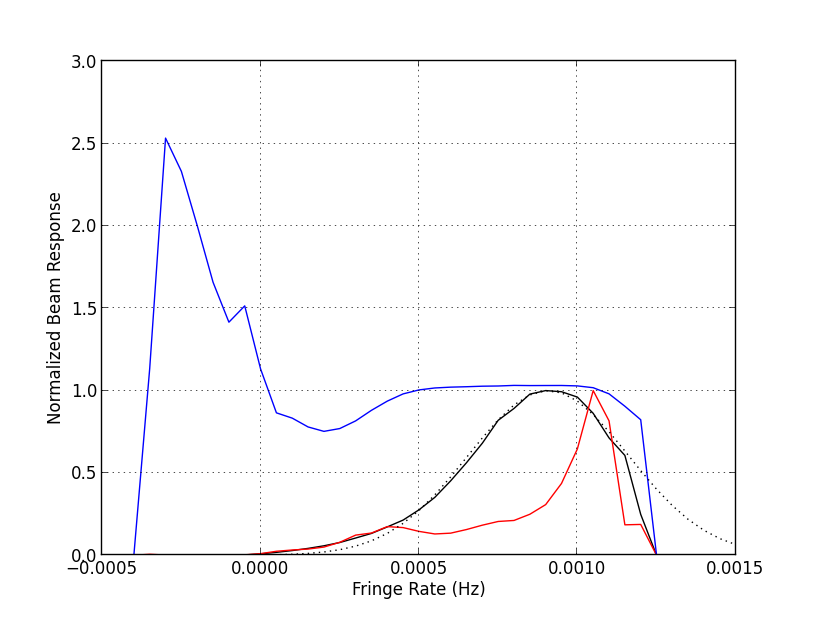
\includegraphics[width=.9\columnwidth]{plots/fringe_wgts.png}
\caption{
}\label{fig:fringe_wgts}
\end{figure}

In order to demonstrate fringe-rate filtering in the applications discussed below, we will make
repeated use of simulated data.  In keeping with its origins targeting observations from the
PAPER array, we choose for our simulations a model array based on PAPER, deployed at a latitude $-30^\circ$
and featuring the beam response pattern characteristic of PAPER dipole elements \citep{parsons_et_al2008,pober_et_al2012}.
For these simulations, we also choose a specific baseline to examine: a pair of antennas separated by 30 m in the 
east-west direction, observing at 150 MHz.  This baseline corresponds to the most repeated (and hence,
most sensitive) baseline length measured by the PAPER array in the maximum-redundancy array configuration it uses
for power spectral measurements \citep{parsons_et_al2012a,parsons_et_al2014,ali_et_al2015}.  As such, this simulation
serves to demonstrate the performance of fringe-rate filtering in the context of the specific instrument configuration
that has been used to place the current best upper limits on 21cm emission from cosmic reionization.

To implement
the fringe-rate filters described below, we begin with the ideal filter shape in fringe-rate space.  In the case 
of the beam-weighted fringe-rate filter described in \S\ref{sec:sim_nos}, this ideal filter shape takes a
truncated Gaussian form where the peak and width have been fit to the projection of the beam model in fringe-rate space,
as illustrated in Figure \ref{fig:fringe_weights}.  
The beam model projection is obtainted
by binning the beam power along fringe-rate contours, as illustrated for coarse fringe-rate bins
in Figure \ref{fig:XXX}.  The analytic Gaussian form is then truncated at the maximum fringe rate to obtain a fringe-rate
filter profile that matches the beam-weighted profile to within a power-averaged RMS of XXX\%.  While it would be possible
to use the beam-weighted profile directly as the ideal fringe-rate filter profile, having an analytic form allows filters
to be rapidly generated as a function of baseline length and observing frequency.  Since optimal SNR weighting is relatively
insensitive small weighting errors (XXX back this up), this level of match between the computed and analytic forms of the
desired fringe-rate filter is acceptable.

The next step in implementing the fringe-rate filter is translating the analytic filter profile in fringe-rate space into 
a time-domain kernel that can be used to convolve the simulated time series of visibilities.  In effect, we implement
the fringe-rate filter as a finite impulse response (FIR) filter.  Applying the fringe-rate filter as an FIR filter in
the time domain, as opposed directly multiplying the desired filter to Fourier-transformed visibilities, has the advantage 
that flagged or missing data can be naturally excluded from the filter by neglecting
FIR taps (coefficient multiplies) that target the missing data. The summed output of the FIR filter are then renormalized to
account for the missing samples.  Another advantage of the FIR implementation of the fringe-rate filter is the potential for
windowing the time-domain filter profile.  While time-domain windowing causes further deviations from the ideal
fringe-rate filter profile, it can be used to produce a more compact time-domain kernel.
Reducing the number of time-domain samples used in the FIR filter improves the computational efficiency of the filter and
helps limit the number of samples potentially corrupted by spurious systematics such as RFI.

To summarize, the simulations are based on a 30-m PAPER baseline observing at 150 MHz.  While the shape of the fringe-rate
filter is application-specific, we generally implement them as FIR filters, with time-domain kernels using coefficients that
are spaced to match the 43-second integrations recorded in our simulated observations.  Finally, we apply an window function to
truncate the wings of this time-domain kernel to increase its compactness in time.  As demonstrated in Figure \ref{fig:fringe_weights},
% XXX add this part to the plot
this windowing increases the power-averaged RMS deviation from the ideal filter to XXX\%, but the improvement in computational cost,
the reduction in impact for any spurious systematics, and the relative insensitivity of the applications described below on the specific
filter shape, make this an advantageous trade-off.

\subsection{Point Source Simulations for Mapping Beam Response}
\label{sec:sim_pnt}

\begin{figure}\centering
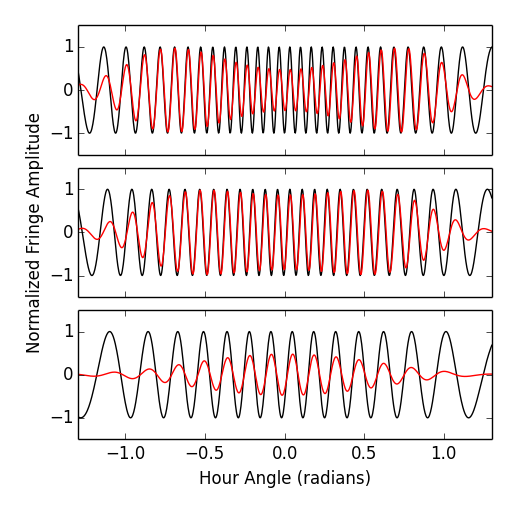
\includegraphics[width=0.9\columnwidth]{plots/src_track.png}
\caption{
Fringe amplitude before (black) and after (red) the application
of the fringe-rate filter described in \S\ref{sec:sim}.  From top to bottom,
the panels illustrate the real component of the visibility measured by
a 30-m east-west baseline deployed at a latitude of $-30^\circ$ 
for point sources 
passing through the fringe pattern at declinations of $0^\circ$,
$-30^\circ$, and $-60^\circ$, respectively.  In this simulation,
antenna elements have isotropic primary beams.
}\label{fig:src_track}
\end{figure}

\begin{figure*}\centering
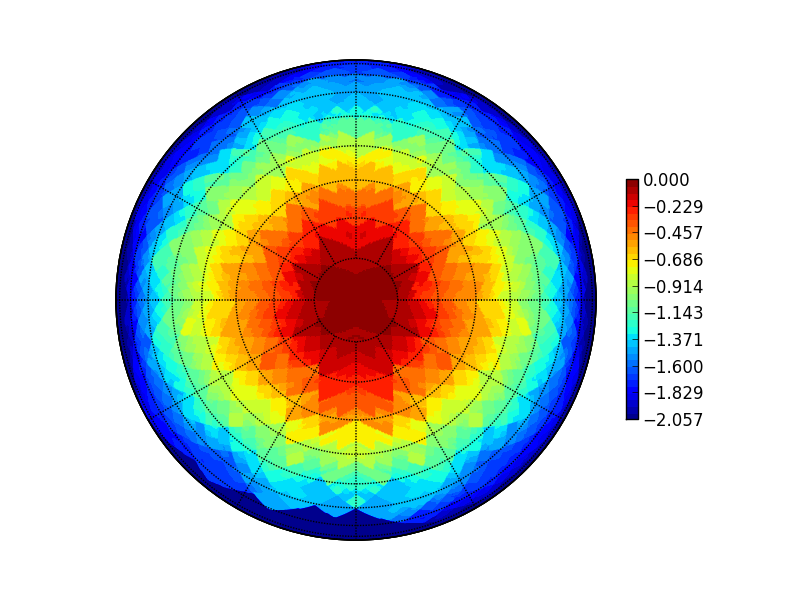
\includegraphics[width=.6\columnwidth]{plots/beam_raw.png}
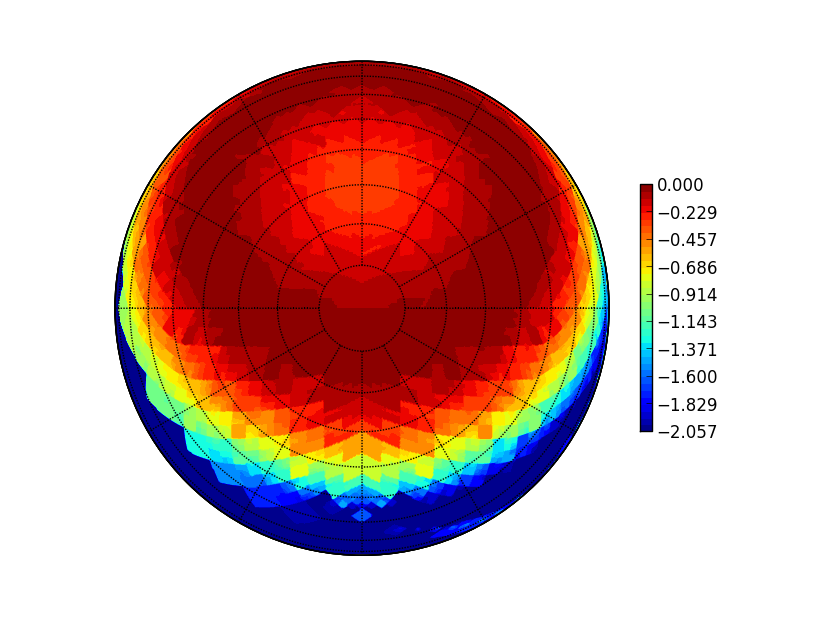
\includegraphics[width=.6\columnwidth]{plots/beam_wgt.png}
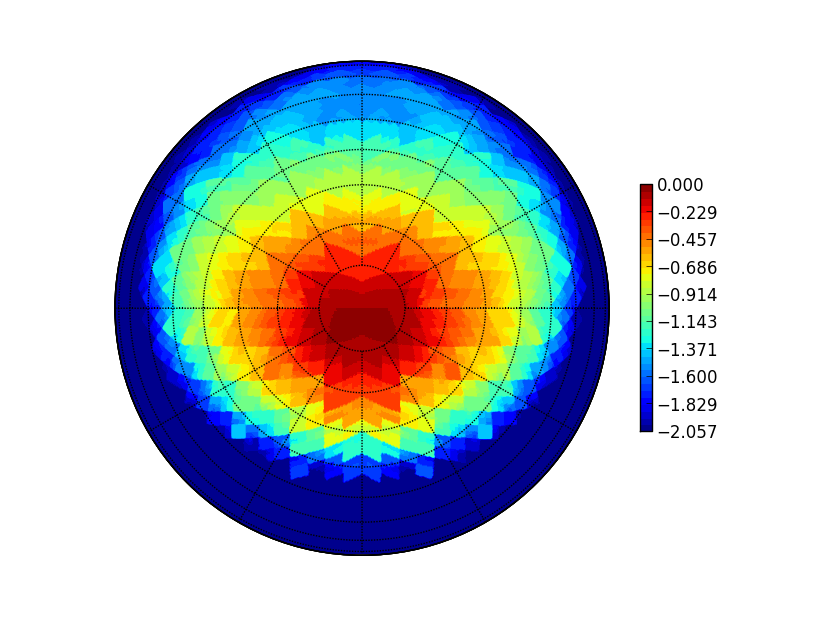
\includegraphics[width=.6\columnwidth]{plots/beam_fng.png}
\caption{
The effective primary beam response of a baseline, as determined from the simulations in \S\ref{sec:sim_pnt}.
Panels indicate reconstructions of PAPER's model beam response used in the simulation (left), the 
beam weighting that results from the application of a fringe-rate filter weighted to optimize SNR for
a 30-m baseline with PAPER's beam response (center), and the effective primary beam response of the
baseline after the application of the fringe-rate filter.
}\label{fig:}
\end{figure*}

\subsection{Optimizing the Signal-to-Noise Ratio in Power Spectral Measurements}
\label{sec:sim_nos}

Specific application for statistically isotropic Gaussian random signals.
Noise Simulations for Determining Effective Volume.

Discuss beam area as normalization that keeps signal level constant.
Refer to \citet{parsons_et_al2014} Appendix A.

We begin by examining the integrated volume, $\mathbb{V}$, used to normalize the 3D Fourier transform in
Equation 3 of P12a. We express this volume in observing coordinates as
\begin{equation}
    \mathbb{V} = \Omega B\cdot X^2Y,
\end{equation}
where $B$ is the bandwidth, $\Omega$ is the angular area, and $X,Y$ are redshift-dependent
scalars relating angle and frequency to spatial scales, respectively.
$\Omega$ arises from the bounds set by $A(l,m,\nu)$, the antenna power response, on the 
angular extent in the integral
\begin{align}
    \Vt^2(u,v,\eta)=&\left(\frac{2k_{\rm B}}{\lambda^2}\right)^2
        \left[\int{dl~dm~d\nu A(l,m,\nu)T(l,m,\nu)e^{-2\pi i(ul+vm+\eta\nu)}}\right]\times\nonumber\\
        &\left[\int{dl^\prime~dm^\prime~d\nu^\prime A^*(l^\prime,m^\prime,\nu^\prime)T^*(l^\prime,m^\prime,\nu^\prime)e^{2\pi i(ul^\prime+vm^\prime+\eta\nu^\prime)}}\right],
\end{align}
which is a slightly modified version of Equation 6 of P12a relating the delay-transformed visibility
$\Vt$, sampled at wavemodes $u,v$ (the Fourier complements of angular coordinates $l,m$) and $\eta$ (the Fourier
complement of spectral frequency $\nu$), to a temperature field $T$.
As shown in XXX, this reduces to
\begin{equation}
    {\tilde V}_{21}^2(u,v,\eta)\approx\left(\frac{2k_{\rm B}}{\lambda^2}\right)^2\frac{B}{X^2Y}
        \widehat P(\k)\int{dl~dm\left|A(l,m)\right|^2}.
\end{equation}

We compare this result with the relation between the delay-transformed visibility,
${\tilde V}$, to the three-dimensional power spectrum of reionization, $P_{21}(\k)$ 
(P12a):
\begin{equation}
    {\tilde V}_{21}^2(u,v,\eta)\approx\left(\frac{2k_{\rm B}}{\lambda^2}\right)^2\frac{\Omega\,B}{X^2Y} \widehat P_{21}(\k).
    \label{eq:v2_vs_pk}
\end{equation}
As this shows, the relevant beam area in Equation \ref{eq:v2_vs_pk} is the
power-square beam, $\Omega_{\rm PP}$, given by
\begin{equation}
\Omega_{\rm PP}\equiv\int{dl~dm\left|A(l,m)\right|^2}.
\label{eq:beam_squared}
\end{equation}
This contrasts with the standard metric for beam area --- the integrated
power beam --- which we will call $\Omega_{\rm P}$, and is given by
\begin{equation}
\Omega_{\rm P}\equiv\int{dl~dm A(l,m)},
\label{eq:beam_area}
\end{equation}
This beam area metric is used to convert visibility measurements from Jy units to mK,
but is incorrect for normalizing power spectra that relate to 
the two-point correlation function of a temperature field.

For equations that relate power-spectrum sensitivity to a system temperature
(e.g. Equations 15 and 16 in P12a)
\begin{equation}
\Omega^\prime\equiv\Omega_{\rm P}^2/\Omega_{\rm PP}
\end{equation}
should be used in lieu of $\Omega$, as
these equations pick up two factors of $\Omega_{\rm P}$ in the conversion from Jy$^2$ to mK$^2$, along with
the a factor of $\Omega_{\rm PP}$ in the denominator relating to the integrated volume.
For equations that relate a measured visibility (in units of brightness
temperature, e.g. Equation \ref{eq:pspec_cosmo}) to $\widehat P(\k)$, the factor of 
$\Omega_{\rm P}^2$ is already 
applied in the conversion from units of Jy to mK, 
and $\Omega$ corresponds to the remaining factor of $\Omega_{\rm PP}$. 

For PAPER, $\Omega_{\rm P}\approx0.72$ sr, while $\Omega_{\rm PP}$ is 0.31 sr.  Following the definition
above, $\Omega^\prime\approx1.69$.  These beam areas are calculated numerically from
a beam model, but typically, $\Omega^\prime$ is about a factor of two larger than $\Omega_{\rm P}$.


Describe simulation, refer to figures, compare results to analytic prediction.

%fringe_rate_filter.py -C psa898_v002 -a cross --clean=1e-2 --minfr=-1 --fr_frac=1.2 

In the last step prior to forming power spectra,
we apply a fringe-rate filter to effect time-domain integration,
using the effective time interval that a baseline measures a single $k$-mode to integrate coherently
(with noise decreasing
as $\sqrt{t}$, in units of mK), before measurements at different times represent independent modes
that must be squared before further integration (with noise now decreasing as $\sqrt{t}$, in units of mK$^2$).

As outlined in Appendix \ref{app:data_compression}
in the context of data compression, we
take the Fourier transform of the time series in each channel and apply a low-pass filter that preserves
fringe-rates that geometrically correspond to sources rotating on the celestial sphere.  
For a planar array with transit observations, fringe-rates vary according to declination, with fringe rates
reaching a maximum ($f_{\rm max}$) at 
$\delta=0^\circ$, decreasing to 0 at $\delta=-90^\circ$, and for an array such as PAPER deployed near
-30$^\circ$ S latitude, reaching a minimum of $\approx-f_{\rm max}/2$ at $\delta=-60^\circ$ on
the far side of the south celestial pole.
In order to
avoid introducing undesirable frequency structure, we apply the same filter, tuned to the width
set by the highest frequency of the sub-band used in the
power spectrum analysis described
in \S\ref{sec:dspec_crossmult}, to each channel,
even though maximum fringe-rates are generally frequency-dependent.
%Since fringe rates are a
%natural basis for celestial emission
%over short time intervals, fringe-rate
%filters can be narrowly tailored to the geometric bounds of a baseline.
%In contrast, simply summing integrations over an equivalent time interval 
%(corresponding to a sinc filter in fringe-rate space) will tend to significantly suppress emission at
%fringe rates that geometrically correspond to the sky.
In a future paper, we will explore the idea
of employing fringe-rate filters that purposely down-weight fringe-rate modes on the sky according to
the expected signal-to-noise ratio in each mode.  Such filters would essentially correspond to a
one-dimensional implementation of the inverse primary beam $uv$-gridding discussed in \citet{morales_matejek2009},
and have many features in common with m-mode synthesis described in \citet{shaw_et_al2013}.

Since thermal noise scatters equally into all fringe rate bins, applying a filter
that passes only fringe rates corresponding the celestial emission has the effect of de-noising the data.
We apply such a filter to the data, choosing the bounds of the filter to match the geometric
bounds set by a 30-m east-west baseline, according to the equation
\begin{equation}
f_{\rm max} = \frac{|\b_{\rm eq}|}{c} \omega_\oplus \nu,
\label{eq:fringe_rate}
\end{equation}
where $f_{\rm max}$ is the maximum fringe rate, 
$\b_{\rm eq}$ is the baseline vector projected parallel to the equatorial 
plane, $c$ is the speed of light,
$\omega_\oplus$ is the angular frequency of the Earth's rotation,
and $\nu$ is the spectral frequency. 
% 780 = 30e2 / c * 2pi / 86164 * .174, where .174 is chosen because want to not attenuate sky over entire band
At 174 MHz (the highest frequency in a 20-MHz window centered on 164 MHz that is used in \S\ref{sec:dspec_crossmult}),
$f_{\rm max}=1.3$ mHz, corresponding to a fringe period of 780 s.  Hence, the fringe-rate filter that is
applied passes fringe-rates in the range $-0.7<f<1.3$ mHz.  The width of this filter corresponds in 
sensitivity to an effective integration time of 525 s.
We note that
this filtering could have been applied during the data compression described in \S\ref{sec:preprocessing},
but was implemented separately to enable the compression to work uniformly
over all baselines in the array without additional information about antenna location.

After applying this filter,
we transform the data back to time domain in preparation for forming power spectra via the delay transform.
It should be noted that, in time domain, the data are now heavily over-sampled; adjacent samples are no longer
statistically independent.  Hence, when averaging power-spectra versus time,
noise will not beat down according to the strict number in samples, but rather, according to
the actual number of statistically independent samples underlying the time series.

\begin{equation}
\widehat P(\k_{t\tau}) = \left(\frac{\lambda^2}{2k_{\rm B}}\right)^2\frac{X^2Y}{\Omega B}
\left\langle{\tilde V_i(\tau,t) \tilde V_j^*(\tau,t)}\right\rangle_{i<j},
\label{eq:pspec_cosmo}
\end{equation}
which follows from equation 12 of P12a, with $\lambda$ being the observing
wavelength, $k_{\rm B}$ is Boltzmann's constant, $X^2Y$ is a cosmological scalar with units
of $\frac{h^{-3}\ {\rm Mpc}^3}{{\rm sr}\cdot {\rm Hz}}$, $\Omega$ is the angular 
area\footnote{
As described in detail in Appendix \ref{app:beam_area}, the angular area used to normalize
high-redshift 21cm power spectrum measurements (e.g., $\Omega$ in Equation \ref{eq:pspec_cosmo}) is proportional
to the integral of the squared beam power over angular area ($\Omega_{\rm PP}$; equation \ref{eq:beam_squared}).
This contrasts the standard beam area ($\Omega_{\rm P}$; equation \ref{eq:beam_area}) that is
used to relate flux density to a brightness temperature.
Since Equation \ref{eq:pspec_cosmo} 
relates a measured visibility in units of brightness
temperature to $P(\k)$, a factor of $\Omega_{\rm P}^2$ has already been
applied to convert Jy to mK.  In this case,
$\Omega$ indicates the remaining factor of $\Omega_{\rm PP}$, which for PAPER is 0.31 sr.},
$B$ is the bandwidth, $\langle\dots\rangle_{i<j}$ indicates the ensemble average
over instantaneously redundant baseline measurements indexed by $i,j$,
and $\tilde V(\tau,t)$ is the delay-transformed visibility,
expressed in terms of delay $\tau$ and time $t$.
We use $t$ as a subscript on $\k$
to denote the different modes sampled by a baseline as the sky rotates, and $\tau$ to indicate
the dependence of $\k$ on the delay mode in question.

\begin{equation}
\widehat \Delta^2_{21}(k) = \frac{k^3}{2\pi^2}\left\langle \widehat P(\k_{t\tau})\right\rangle_{|\k_{t\tau}|=k},
\end{equation}
where the three-dimensional symmetry of the power spectrum is invoked to average over
all independent measurements of modes in a shell of $|\k|=k$, with independent measurements
indexed here by $t$.  As described in \S\ref{sec:fringe_rate_filtering}, the number of independent modes
that are averaged (with noise decreasing with number of modes, $M$, as $\sqrt{M}$ in mK$^2$ units; see P12a) is 
determined
by overall observing window and the number of fringe-rate bins that are 
preserved in the fringe-rate filtering process.
Since we have not decimated the number of integrations to the critical sampling rate corresponding to the 
width of the applied fringe-rate filter, $M$ is {\it not} the number of integrations.  However,
we are free to average the power spectrum estimates for each integration, even though nearby samples
do not have statistically independent noise, understanding that noise will decrease according to the number
of underlying independent samples.


\subsection{Polarization Response}
\label{sec:polbeams}
\def\VXX{{V_{\rm XX}}}
\def\VYY{{V_{\rm YY}}}
\def\VI{{V_{\rm I}}}
\def\VQ{{V_{\rm Q}}}

\begin{figure*}\centering
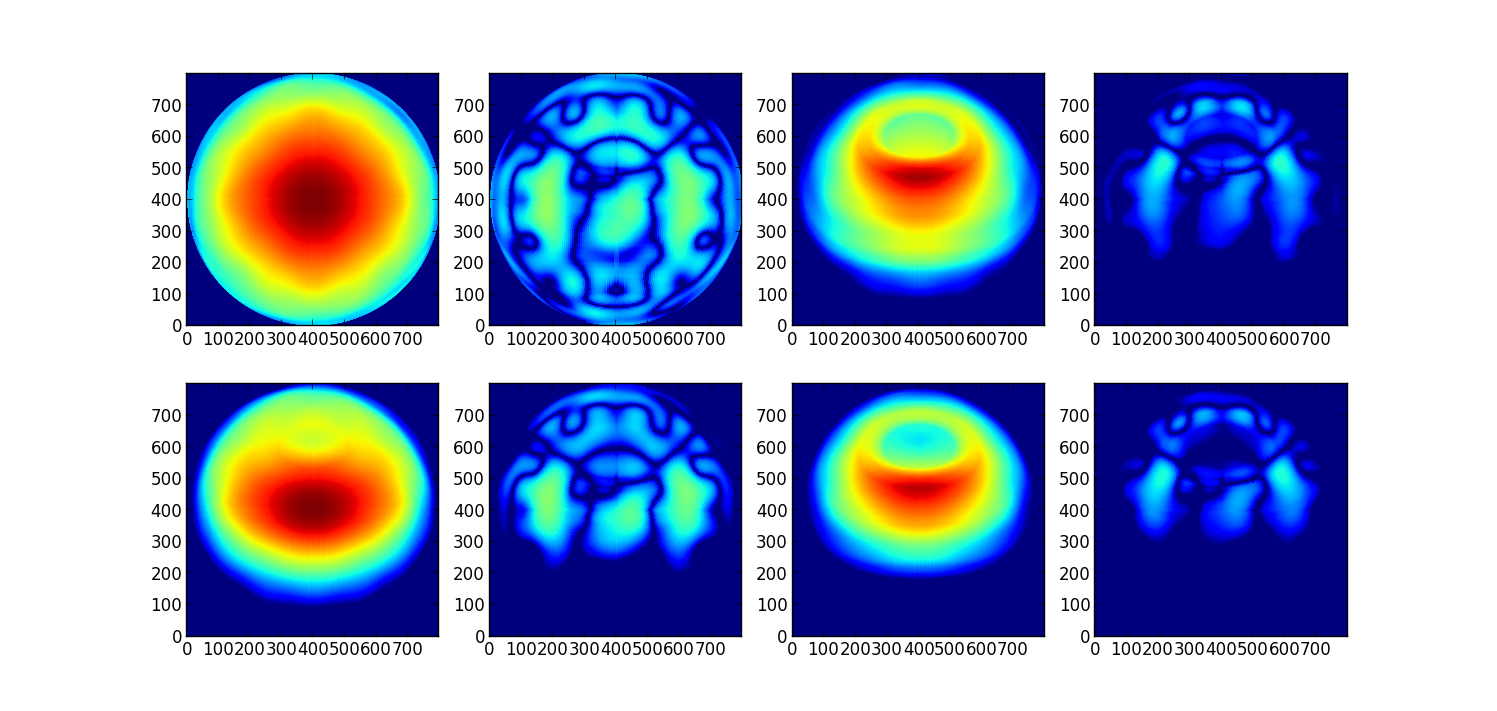
\includegraphics[width=.9\columnwidth]{plots/fringe_beam_wgts.png}
\caption{
}\label{fig:fringe_beam_wgts}
\end{figure*}


Minimizing cross-contamination between Stokes terms in interferometric polarization measurements
is of paramount importance for 21cm cosmology experiments that rely on
the spectral axis to probe the line-of-sight direction at cosmological distances.  For these
experiments, Faraday rotation combines
with a spurious coupling between Stokes terms (typically Q to I) to produce polarization leakage whose 
spectral structure poses a worrisome foreground
to the cosmological signal \citep{jelic_et_al2008,bernardi,moore_et_al2013,moore_et_al2015}.  Current interferometers
targeting the 21cm signal at cosmological distances (LOFAR, MWA, PAPER, HERA, CHIME, LEDA) all employ linearly
polarized feeds, primarily because of their ease of construction and ability to co-locate elements sensitive to
orthogonal polarizations.  However, orthogonal linearly polarized feeds in practice have primary beam responses
that do not match.  As described in \citet{moore_et_al2013}, if left uncorrected, the unmatched beam response 
between visibilities $\VXX$ and $\VYY$ measuring the XX and YY polarization products, respectively, is the 
dominant source of polarization leakage in the Stokes I measurement $\VI\equiv(\VXX+\VYY)/2$ for
linearly polarized feeds.

With an accurate beam model, it is trivial to rescale $\VXX$ and $\VYY$ 
so that the XX and YY beam responses match in a chosen (typically, zenith) direction.  Their sum, $\VI$, then
represents a perfect probe of the Stoke I parameter in that chosen direction, but will contain contamination
from $\VQ\equiv(\VXX-\VYY)/2$ in directions where the XX and YY beam responses do not match.
The heart of the problem is the impossibility of creating a match between a pair of two-dimensional functions (the
XX and YY beam responses) with a single degree of freedom (the amplitude of $\VXX$ relative to $\VYY$).  In order
to improve the match between polarization beams in interferometric measurements, many interferometric measurements
from distinct points in the UV plane will have to be combined with appropriate weights to effect a reweighting
of the sky along two dimensions.

The typical technique for correcting the mismatch between the XX and YY polarization beams is to separately
image these polarization products, correct each pixel in each image using modeled beam responses,
and then to sum the corrected images together to form a Stokes I map 
(e.g. \citealt{sullivan,lofar,bernardi}).  Mathematically, this technique is identical to convolving the sampled
UV plane by the Fourier transform of the directionally-dependent correction applied in image domain, and for an ideal
array that samples the UV plane at scales significantly finer than the aperture of a single element, this technique can
in principle perfectly correct mismatches between the XX and YY polariation beams.
However, the success that can be achieved with this technique depends strongly on an array's UV sampling pattern.

Take, for example, the case of a sparsely sampled UV plane where the spacing between UV samples is much greater than
the aperture scale of a single element.  In this case, the beam correction described above 
convolves each UV sample with a kernel kernel whose size scales roughly as the size of the aperture of a
single element in wavelengths.  Since this kernel is much smaller than the spacing between UV samples, 
each point in the convolved UV plane is dominated by the product of a kernel weight and a single visibility measurement.
As such, for a chosen UV coordinate, the level of leakage in the Stokes I UV plane can
be no better than what can be achieved by using a single number to rescale $\VXX$ and $\VYY$ before summing.  

For cases where UV sampling falls somewhere between the sparse and the oversampled cases described above, the level
of primary beam correction that can be realized is more complicated.  Ultimately, the Fourier relationship between
the UV plane and the image dictates that samples that are nearby to one
another in the UV plane enable primary beam corrections on the largest angular scales, while samples that are farther
apart contribute to corrections on finer angular scales, with the orientation of the samples relative to one another
dictating the axis along which such corrections take effect in image domain.  Typically, earth-rotation synthesis
is required to sample the UV plane densely enough to allow for effective beam correction, although some array
configurations are not dense enough to fully correct the beam even then.  One particularly relevant case that falls
in this last category are many of the maximum redundancy configurations currently favored by several 21cm cosmology experiments
for their sensitivity benefits \citep{parsons_et_al2012a,parsons_et_al2014}.

However, even in the single-baseline case, earth-rotation synthesis provides dense UV sampling along one direction --- the
direction the baseline traverses in the UV plane as its project toward the phase center changes.  The appropriate
convolution kernel can combine samples along this track so as to correct the primary beam mismatch along one axis.
It should not surprise the reader that what we have just described --- a convolution kernel acting along a time series
of samples from a single baseline --- is an alternate description of fringe-rate filtering.  Through the correct
choice of fringe-rate filter, it is possible to improve the match between the XX and YY polarization beams, and
in the case of sparse array sampling, the result will be identical to the best that can be achieved by independently
imaging the polarization products.  While this is not as effective at mitigating polarization leakage as can be achieved
through imaging in the dense sampling case, we show in \S\ref{sec:XXX} that it nonetheless represents a substantial improvement
over the naive summing of XX and YY visibility measurements.

% XXX discuss results here 

\subsection{Instrumental Systematics and Off-Axis Foregrounds}
\label{sec:foregrounds}

% XXX cite ellingson somewhere?  what does his paper say?

A final application of beam sculpting with fringe-rate filters targets the suppression of systematics in data.
We will consider two systematics: additive phase terms associated with instrumental crosstalk, and sidelobes
associated with celestial emission outside of the primary field of interest.  Both of these applications are 
closely aligned with the original application of fringe-rate filters described in \citet{parsons_backer2009}.

For the purposes of this discussion, we consider instrumental crosstalk to be a spurious 
correlation introduced between otherwise uncorrelated signals
as a result of electromagnetic coupling in the instrument (typically between adjacent, unshielded signal lines)
or because a non-celestial source has injected a correlated signal (e.g. switching noise on power supplies).
Although crosstalk can be suppressed using Walsh switching (XXX cite), it is always present at some level
in interferometric observations.  If it is temporally stable, however, it is possible to significantly
suppress crosstalk in data by averaging visibilities over a long period (so that the fringing celestial
signal washes out) and then subtracting the average complex additive offset from the data.  This 
technique has
long been applied to, e.g., PAPER observations \citep{parsons_et_al2010,jacobs_et_al,pober_et_al,parsons_et_al2014}.

As a time-domain filter, this crosstalk removal technique can also naturally be understood as a notch filter
for removing signals with zero fringe-rate.  Because crosstalk removal uses a finite time interval for computing
the average, applying this notch fringe-rate filter has the effect of removing emission from the region of
sky corresponding to the zero fringe-rate bin.  As illustrated in Figure \ref{fig:fringe_contours}, for
a 30-m baseline observing at 150 MHz, this corresponds to the unshaded region intersecting the south celestial pole.
For PAPER, this region is sufficiently low in the beam that its removal has little impact, but in general, 
subsequent analysis of crosstalk-removed data may require accounting for the beam-sculpting effects of
the crosstalk removal filter.

Thus, when considering instrumental systematics, there may be additional criteria that influence one's
choice of fringe-rate filter besides optimizing signal-to-noise; one may choose to excise the zero fringe-rate
bin to improve data quality at a very modest cost to sensitivity.  Similarly, it is common to encounter situations
where celestial emission that is low in the primary beam is bright enough to introduce undesireable 
sidelobe structure or other systematics in observations targeting an area nearer to beam center.  In this case,
one may again find it desireable to depart from optimal SNR weighting in a fringe-rate filter
% XXX check SNR is defined
by further down-weighting regions of low sensitivity in order to gain improvements in foreground systematics.
This application of fringe-rate filtering is particularly relevant for 21cm cosmology experiments where approximately
Gaussian signals are overlaid with highly non-Gaussian foregrounds.  Fringe-rate filters that are informed by 
the angular structure in foreground models can substantially suppress foreground systematics while having little
impact on a statistically isotropic Gaussian signal.

%XXX add a simulation for this?

%\begin{figure*}\centering
%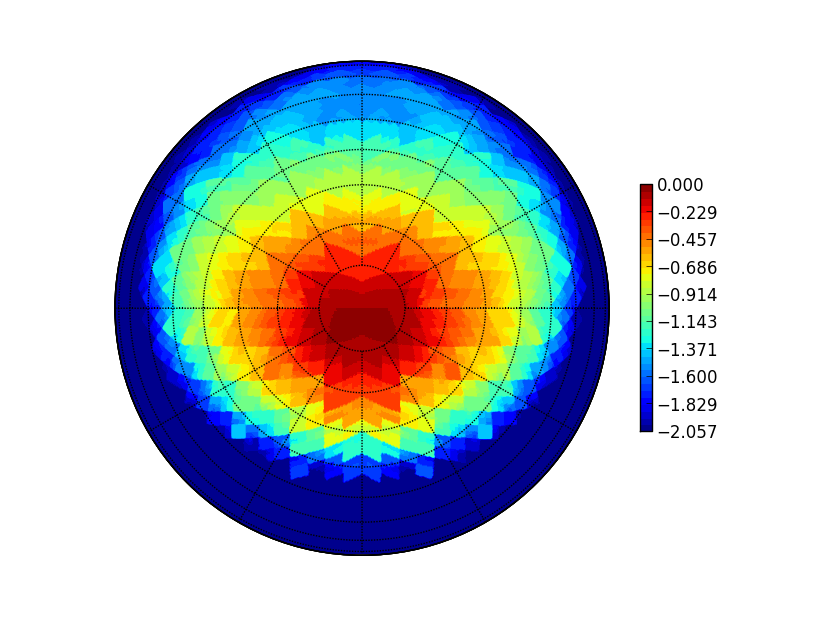
\includegraphics[width=.6\columnwidth]{plots/beam_fng.png}
%\caption{
%The effective primary beam response of a baseline, as determined from the simulations in \S\ref{sec:sim_pnt}.
%Panels indicate reconstructions of PAPER's model beam response used in the simulation (left), the 
%beam weighting that results from the application of a fringe-rate filter weighted to optimize SNR for
%a 30-m baseline with PAPER's beam response (center), and the effective primary beam response of the
%baseline after the application of the fringe-rate filter.
%}\label{fig:}
%\end{figure*}


%\section{Discussion}
%\label{sec:results}

%Before/after power spectrum plot.
%FR transform of real data.
%Application of FR filter to waterfall.  

\section{Conclusion}
\label{sec:conclusion}

In this paper, we have revisited the concept of filtering the visibility time-series
measured by an interferometric baseline that was presented in \citet{parsons_backer2009}.
Using a mapping between the timescale of variation in visibility data and position
on the sky for a chosen baseline, we show that the rectangular time windows typically
used when integrating visibilities are almost always sub-optimal, and motivate 
filtering on the basis of fringe rate
as step for optimally combining time-ordered visibility data.  In \S\ref{sec:XXX}, we show 
that fringe-rate filtering indeed can represent a computationally efficient first step
for optimal mapmaking, particularly for telescopes with sparsely sampled apertures, or
for interferometers with wide fields of view where gridding in the UV plane incurs a significant
computational cost.

We also show that fringe-rate filtering can alternately be interpreted as a per-baseline
operation for sculpting the primary beam along the declination direction.  Using analytic
derivations and simulations, we highlight several important applications of such beam
sculpting.  One key application for 21cm cosmological experiments starved for sensitivity
is the ability to re-weight visibility data according to the SNR in each fringe-rate bin.
This operation, which is effectively a one-dimensional case of the optimal beam
weighting described in \citet{morales_matejek2009} and \citet{bhatnagar_et_al2008}, 
can improve the sensitivity achieved in a per-baseline power spectral analysis by a factor
of several % XXX check
while avoiding many of the systematics associated with gridding data in the UV plane.
Other important application include improving the match between polarization beam to
reduce polarization leakage, and down-weighting areas low in the primary beam
to reduce systematics from off-axis foregrounds.

In \citet{ali_et_al2015}, the fringe-rate filtering techniques presented here are applied to
observations from the PAPER array as part of their power-spectrum analysis pipeline.  The
results highlight the power of fringe-rate filtering in 21cm cosmology applications.
Given its efficiency, flexibility, and close alignment with the natural observing
basis of radio interferometers, we anticipate that fringe-rate filtering is likely to be
an important analysis tool for current 21cm experiments, as well as future instruments
such as the Hydrogen Epoch of Reionization Array (HERA; \citealt{pober_et_al2014}) and
the Square Kilometre Array (SKA; \citealt{XXX}).


\section{Acknowledgment}

It gives us great pleasure to thank James Aguirre, David Moore, Danny Jacobs, 
Miguel Morales, and Jonathan Pober for helpful discussions.  This research
was supported by the National Science Foundation, award \#1129258.

% ---------------------------------------------------------------------
% ---------------------------------------------------------------------
% ---------------------------------------------------------------------

%\clearpage
\bibliographystyle{apj}
\bibliography{biblio}

\end{document}

